%%%%%%%%%%%%%%%%%%%%%%%%%%%%%%%%%%%%%%%%
% University/School Laboratory Report
% LaTeX Template
% Version 3.1 (25/3/14)
%
% This template has been downloaded from:
% http://www.LaTeXTemplates.com
%
% Original author:
% Linux and Unix Users Group at Virginia Tech Wiki 
% (https://vtluug.org/wiki/Example_LaTeX_chem_lab_report)
%
% License:
% CC BY-NC-SA 3.0 (http://creativecommons.org/licenses/by-nc-sa/3.0/)
%
%%%%%%%%%%%%%%%%%%%%%%%%%%%%%%%%%%%%%%%%%

%----------------------------------------------------------------------------------------
%   PACKAGES AND DOCUMENT CONFIGURATIONS
%----------------------------------------------------------------------------------------

\documentclass{article}

\usepackage[version=3]{mhchem} % Package for chemical equation typesetting
\usepackage{siunitx} % Provides the \SI{}{} and \si{} command for typesetting SI units
\usepackage{graphicx} % Required for the inclusion of images
\usepackage{natbib} % Required to change bibliography style to APA
\usepackage{amsmath} % Required for some math elements 
\usepackage{listings}
\usepackage{float}
\usepackage[center]{caption}
\usepackage{enumerate}
\usepackage{soul}
\usepackage{csquotes}
\usepackage{tcolorbox} 
\usepackage{minted}
\usepackage{hyperref}

%\setlength\parindent{0pt} % Removes all indentation from paragraphs

%\renewcommand{\labelenumi}{\alph{enumi}.} % Make numbering in the enumerate environment by letter rather than number (e.g. section 6)

%\usepackage{times} % Uncomment to use the Times New Roman font

%----------------------------------------------------------------------------------------
%   DOCUMENT INFORMATION
%----------------------------------------------------------------------------------------

\date{\today} % Date for the report

\begin{document}
% Define document title and author
\title{Fourier Methods}
\author{Johnny Pribyl}
\markboth{Montana State University}{}
\maketitle

\begin{abstract}

    This lab is designed to familiarize the student with thinking in the
    frequency domain. It requires far more data collection than the previous
    labs. There are four main objectives. First, we worked with a few simple
    input functions in order to become familiar with the spectrum analyzer.
    Second, we investigated the response of an LRC circuit to several different
    signal types. Third, we did the same thing to an acoustical cavity. And
    lastly, we examined a system of coupled torsional reed oscillators.
    Unfortunately, we ran out of time and were not able to collect all of the
    necessary data from the reed oscillators - so, this report will only
    include an informal discussion of theory and observed results.
    
\end{abstract}



%----------------------------------------------------------------------------------------
%   SECTION 1
%----------------------------------------------------------------------------------------
\section{Introduction}

Somehow, every undergraduate physics student manages to sneak through their
classes without ever fully understanding Fourier methods. Brian took it upon
himself to fill this educational hole with experimental knowledge. That means
this lab operates almost entirely in the frequency domain. Or, in other words,
we Fourier Transform \textit{everything}.

Although it's pretty tough to get funding these days, MSU still has some toys
leftover from the 90s. Among those is the SR770 Spectrum Analyzer. It boasts a
peaceful green-hued digital output and the capacity to live stream the
frequency domain of a time-dependent signal. It only lacks the phrase
\textit{\textbf{DON'T PANIC.}} Ideally, this would be inscribed in large
friendly letters on its cover.

We used the SR770 and TBS1052B-EDU oscilloscope extensively in this lab. Both
of them are capable of saving hundreds of data points at the press of a button.
So, we had quite a bit more real data to analyze for this lab than we have had
for any of our previous forays.

As before, you can find all of my code and data at:
\begin{verbatim}
    jpribyl/cautious-palm-tree
\end{verbatim}

\subsection{Database Design}%

The majority of this lab's data is relatively straightforward. Typically there
are two columns - one for the dependent variable (say, voltage) and one for the
independent variable (typically time or frequency). We saved this data into
.csv files on a USB. However, all of the measurements carry a large amount of
metadata regarding input frequency, amplitude, channel, and the source of the
data. Unfortunately, all of the metadata is not recorded into the files. We
wrote it all down in our lab notebooks, but that makes it difficult to cross
reference.

It would definitely be possible to store all the time / voltage data in excel
and assign values to the metadata with python as we read it in. However, that
approach does not scale very well. It's particularly ineffective for
collaborative efforts. Ideally, there would be a way to tie all of the
metadata to the files themselves. This ensures data integrity without
requiring all collaborators to use an identical code base. It turns out, I'm
not the first person in the world who has had this problem. The correct tool
for the job is a ``database." 

Databases are created and maintained with a language called SQL, or Structured
Query Language. Every measurement is given a unique identifier that allows
anyone to access or ``query" all of its metadata.

Our data did not come pre-packaged with unique identifiers, so I had to add
them manually. Bash has several incredibly powerful text-editing commands that
are perfect for this kind of task. I'm not as familiar with Awk, so I opted to
use Sed. If you have a bash shell on your computer you should be able to access
the man pages with 

\begin{verbatim}
    man sed
\end{verbatim}

Otherwise, you can read them online at gnu.org/software/sed/manual/sed.txt. The
first step was collecting all of our files into a single directory and naming
them numerically so that I can sort through them with a for loop:

\begin{figure}[thp]
\centering
\begin{minipage}{.8\textwidth}
\begin{tcolorbox}
\begin{minted}{bash}
    #!/bin/bash
    cur_id=1;

    for i in $(ls * | sort -V);
    do
        echo $i
        echo $cur_id

        #double quotes allow variables
        sed -i "s/\(.*\)/$cur_id,\1/" $i

        let cur_id+s=1
    done
\end{minted}
\end{tcolorbox}
\end{minipage}
\end{figure}

I find bash incredibly hard to read, so let's break this down a bit. The very
first line is known as a ``shebang" and tells the computer to use bash for this
script. Next I define a variable ``cur\_id" which holds the unique
identifier that will get prepended to every line of the data files.

After that I run through every file in the current directory and sort them
``naturally." For each file, I read out (or echo) the file name and the file's
identifier. Then, I tack the current id and a comma in front of every line in
the file and increment the cur\_id by 1.

Let's say that the first file in a given directory looks like this:
\begin{figure}[thp]
\centering
\begin{minipage}{.8\textwidth}
\begin{tcolorbox}
\begin{minted}{python} 
    0.0000000e+000, -1.3732910e-001,
    6.2500000e+001,  9.4042969e+000,
    ...
    1.2500000e+002, -4.9438477e-002,
    1.8750000e+002, -7.1411133e-002,
    2.5000000e+002, -3.2958984e-002,
    3.1250000e+002, -3.2958984e-002,
\end{minted}
\end{tcolorbox}
\end{minipage}
\end{figure}

My script will turn it into something that looks like this:
\begin{figure}[thp]
\centering
\begin{minipage}{.8\textwidth}
\begin{tcolorbox}
\begin{minted}{python} 
    1,  0.0000000e+000, -1.3732910e-001,
    1,  6.2500000e+001,  9.4042969e+000,
    ...
    1,  1.2500000e+002, -4.9438477e-002,
    1,  1.8750000e+002, -7.1411133e-002,
    1,  2.5000000e+002, -3.2958984e-002,
    1,  3.1250000e+002, -3.2958984e-002,
\end{minted}
\end{tcolorbox}
\end{minipage}
\end{figure}

Where 1 is the unique identifier for this measurement. The second file in the
directory would look very similar except that it would be prepended with a 2
instead of a 1. 

After pre-processing the data, I read it into my database. If you want to play
with the database at home, you can restore it using MySQL Workbench from the
dump files in 

\begin{verbatim}
    lab3/data/database/databasedump
\end{verbatim}

If you don't feel like downloading my database, I really wouldn't blame you.
It's not exactly anything groundbreaking. Besides, I took the 30 seconds
required to generate an EER diagram mapping the relationships between tables.
I'll let you peruse it at your leisure.

\begin{figure}[H]
\begin{minipage}{1.12\textwidth}
\begin{tcolorbox}
    \centering
        % Center the figure.
        % Include the eps file, scale it such that it's width equals the column width. You can also put width=8cm for example...
        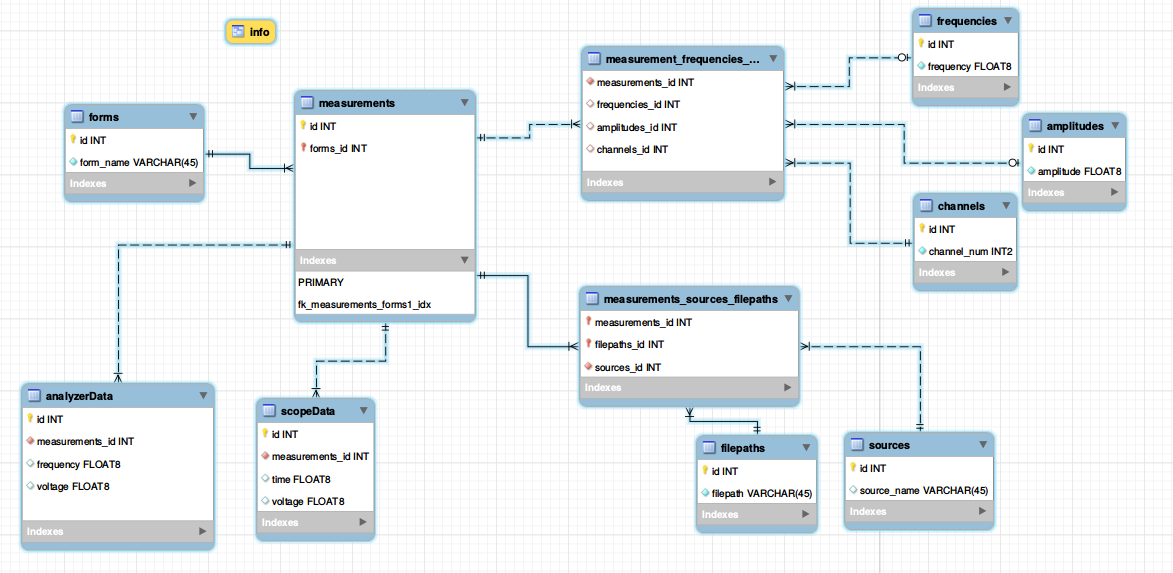
\includegraphics[width=12.5cm, height=6cm]{figures/figure1.png}
        % Create a subtitle for the figure.
        \caption{EER diagram mapping the database}
        % Define the label of the figure. It's good to use 'fig:title', so you know that the label belongs to a figure.
        \label{fig:fig1}
\end{tcolorbox}
\end{minipage}
\end{figure}

The little yellow box entitled ``Info" corresponds to a view, or saved query
that allows for easier access to the desired data without sacrificing the
structure of an ACID database. If you were to run a simple query on the view:

\begin{figure}[H]
\centering
\begin{minipage}{.4\textwidth}
\begin{tcolorbox}
\begin{minted}{sql}
select * from info
\end{minted}
\end{tcolorbox}
\end{minipage}
\end{figure}
%\begin{verbatim}
    %SELECT * FROM info
%\end{verbatim}

You would get something back that looks like:
\begin{figure}[H]
\begin{minipage}{1.12\textwidth}
\begin{tcolorbox}
    \centering
        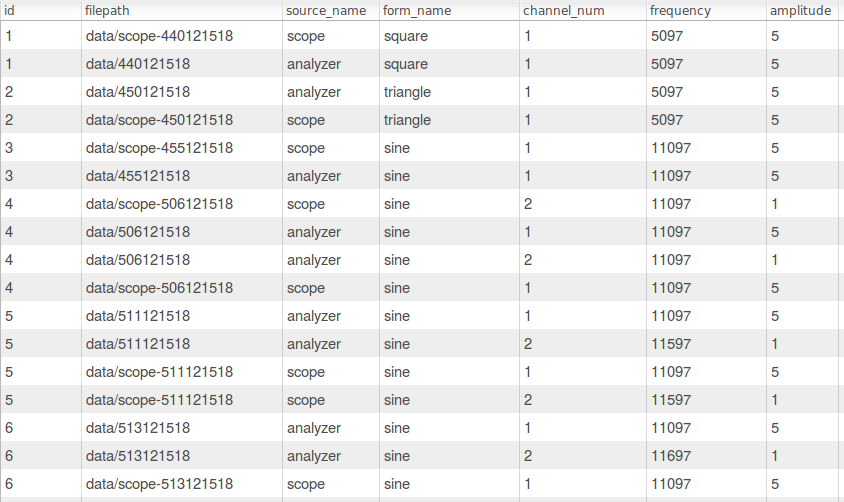
\includegraphics[width=8.9cm, height=5.3cm]{figures/figure2.png}
        \caption{A simple query on the database}
        \label{fig:fig2}
\end{tcolorbox}
\end{minipage}
\end{figure}

Hopefully all of that made sense. If not, don't worry about it -- it's not really
too relevant to the actual data analysis.
%----------------------------------------------------------------------------------------
%   SECTION 2
%----------------------------------------------------------------------------------------
\section{Objectives}

All of these labs have objectives instead of procedures. They are intended to
guide our experiments without spoon feeding us the results. Sometimes I really
miss eating bananas out of a jar. Fortunately for me, most grocery stores still
stock Gerber snacks. 

If you're not familiar with the methods and procedures of this lab, then I
would suggest reviewing the manual. It is quite extensive and details all the
theory far more eloquently than I ever could. It lives in:

\begin{figure}[H]
\centering
\begin{minipage}{.8\textwidth}
\begin{tcolorbox}
\begin{minted}{bash}
lab3/lab_descrip/Fourier_Methods_manual.pdf
\end{minted}
\end{tcolorbox}
\end{minipage}
\end{figure}

\subsection{Introduction to Spectrum Analyzers}

The first thing we did in lab after putting our heads on straight was run a few
single frequency waves through the oscilloscope and spectrum analyzer. The goal
of this section was to get comfortable with the conversion between frequency
and time domains. All of the oscilloscope data lives in the time domain.
This means that time is the independent variable and our plots consider
$Voltage(time)$. However, it is often useful and always didactic to convert
this data into $V(\omega)$ by Fourier Transforming it:

\begin{equation}
    X(\omega) = \int_{-\infty}^{\infty} x(t) e^{-i \omega t} dt
\end{equation}

Technically, we have a discreet data set that isn't quite infinite, so it might
be more accurate to say that we are using a Fourier Series -- but the theory is
extremely similar and a full discourse on Fourier Analysis is outside of the
scope of this report.
\subsubsection{Sine, Square, and Triangle Waves}%
\label{ssub:sine_square_and_triangle_waves}


If we use the function generator to produce a Sine wave of 11,097 Hz, we get a
familiar looking graph of $V(t)$ on the scope:

\begin{figure}[H]
    \centering
\begin{minipage}{10cm}
\begin{tcolorbox}
        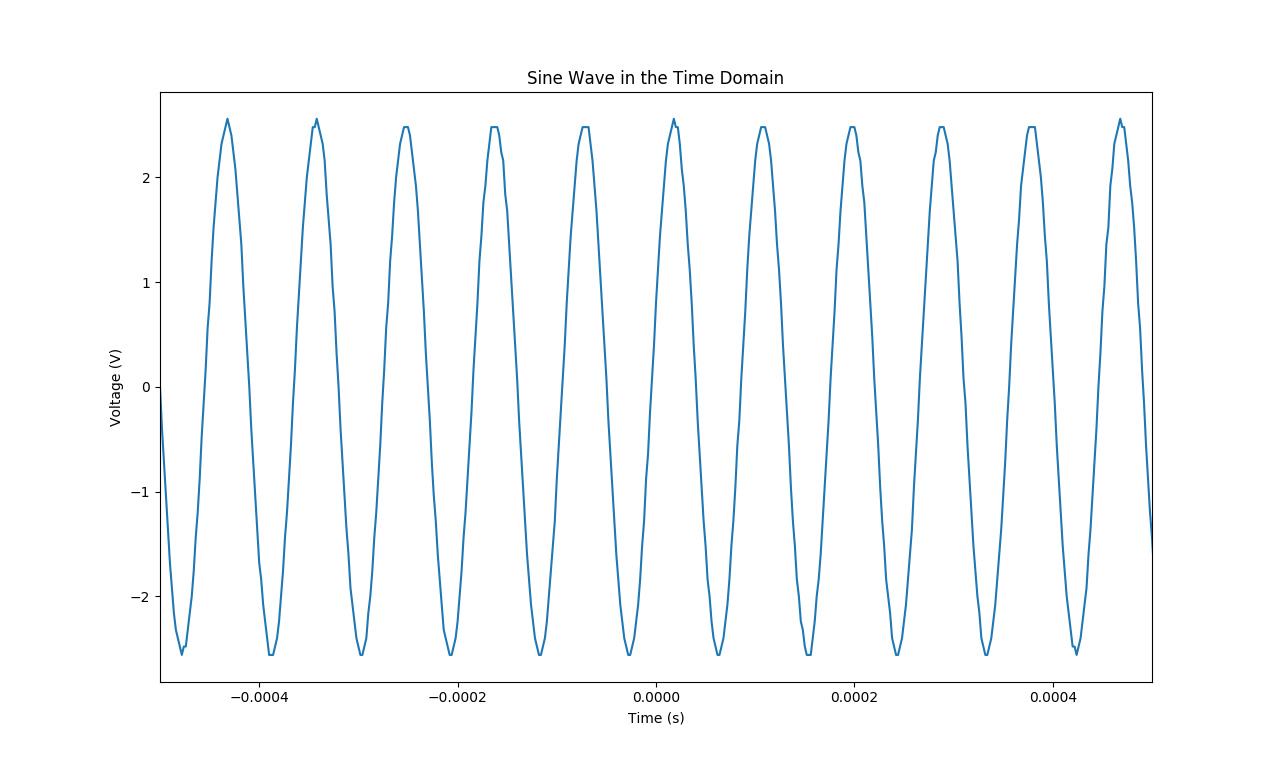
\includegraphics[width=9cm, height=5.cm]{figures/figure3.png}
        \caption{Sine wave of 11.097 kHz collected from the oscilloscope}
        \label{fig:fig3}
\end{tcolorbox}
\end{minipage}
\end{figure}

Now, everyone knows that the Fourier Transform of a sine wave is a delta
function so let's transform the data that we collected from the scope and see
how it looks:

\begin{figure}[H]
    \centering
\begin{minipage}{10cm}
\begin{tcolorbox}
        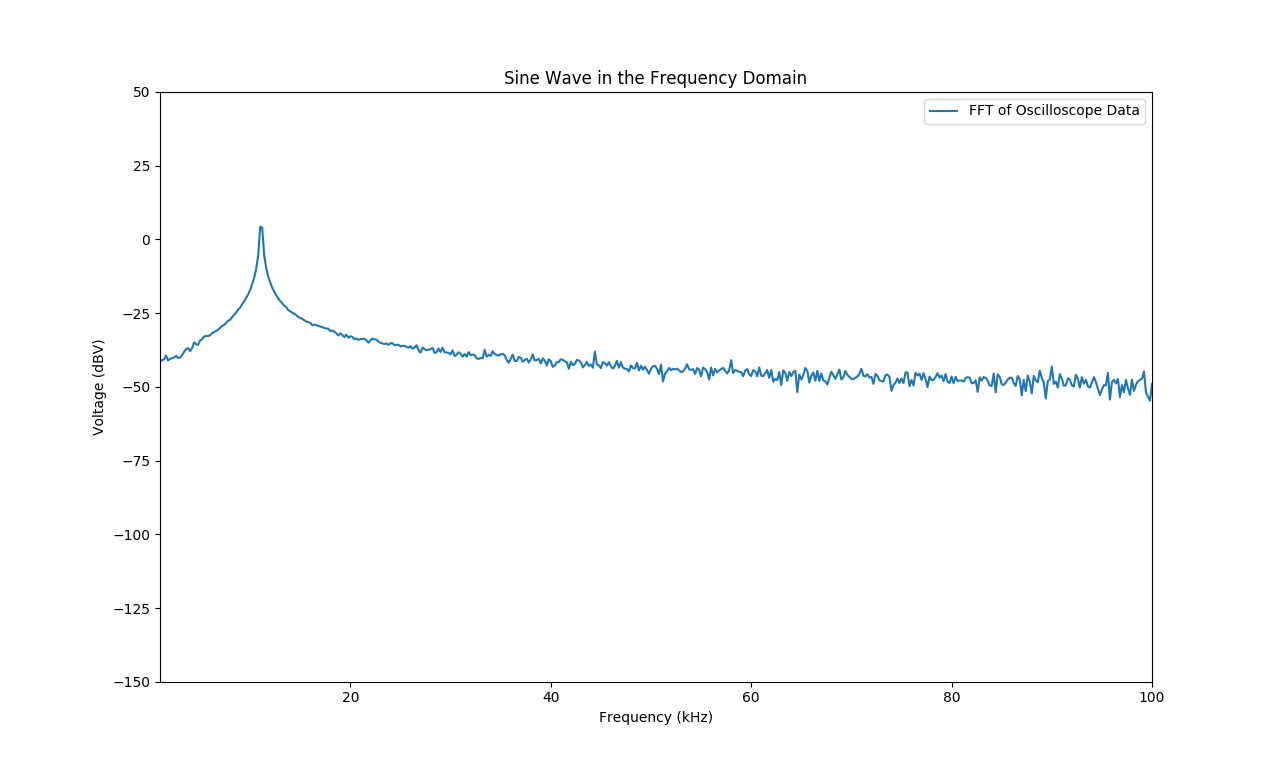
\includegraphics[width=9cm, height=6.5cm]{figures/figure4.png}
        \caption{FFT of data presented in Figure 3}
        \label{fig:fig4}
\end{tcolorbox}
\end{minipage}
\end{figure}

As you can see, there is a single peak at 11.097 kHz. So far, it seems like all is well in the world, but let's overlay the results
with the data collected from the SR770 and see whether things actually match
up.

\begin{figure}[H]
    \centering
\begin{minipage}{11cm}
\begin{tcolorbox}
        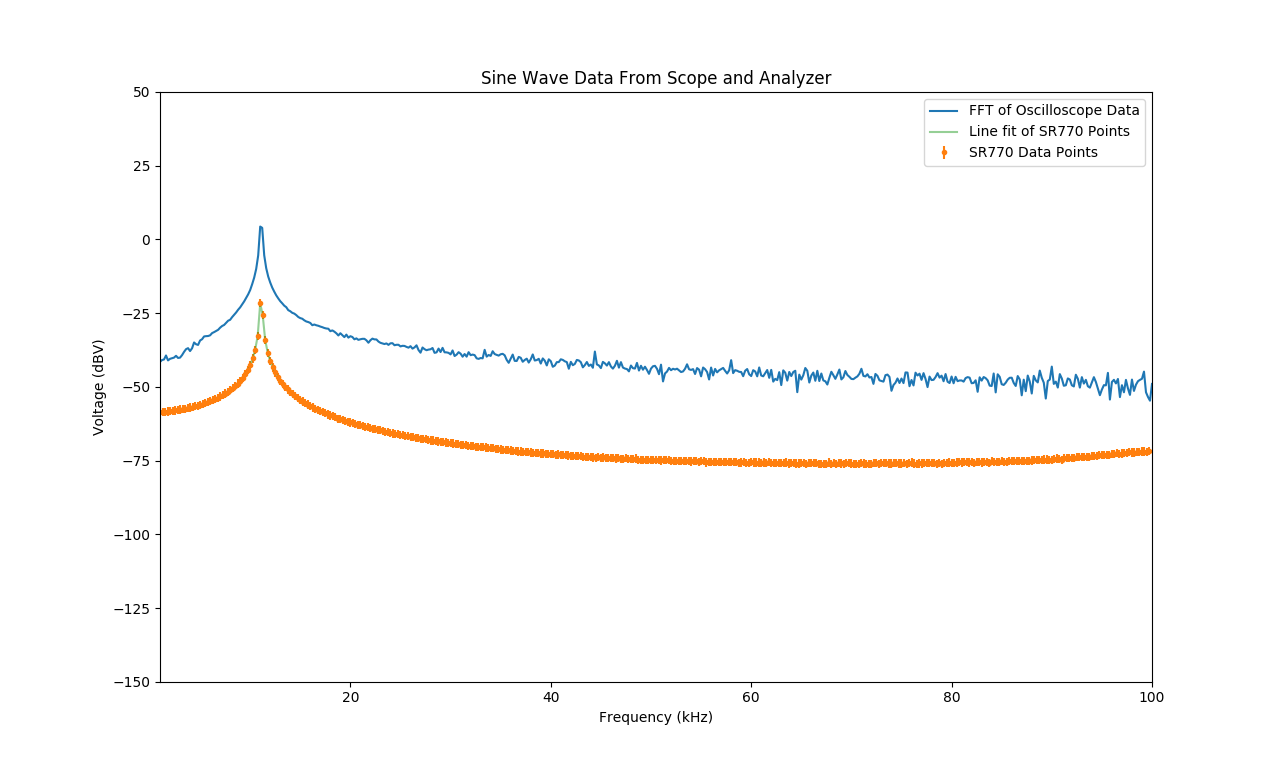
\includegraphics[width=10cm, height=6.cm]{figures/figure5.png}
        \caption{Analyzer data overlaid on top of Figure 4}
        \label{fig:fig5}
\end{tcolorbox}
\end{minipage}
\end{figure}

The last thing to do before moving on is model the results. The plot is
starting to get a little bit busy, but modeling a sine wave is quite easy. All
we have to do is plug in the frequency, transform a vector of points, and
overlay the final plot in the series:

\begin{figure}[H]
    \centering
\begin{minipage}{11cm}
\begin{tcolorbox}
        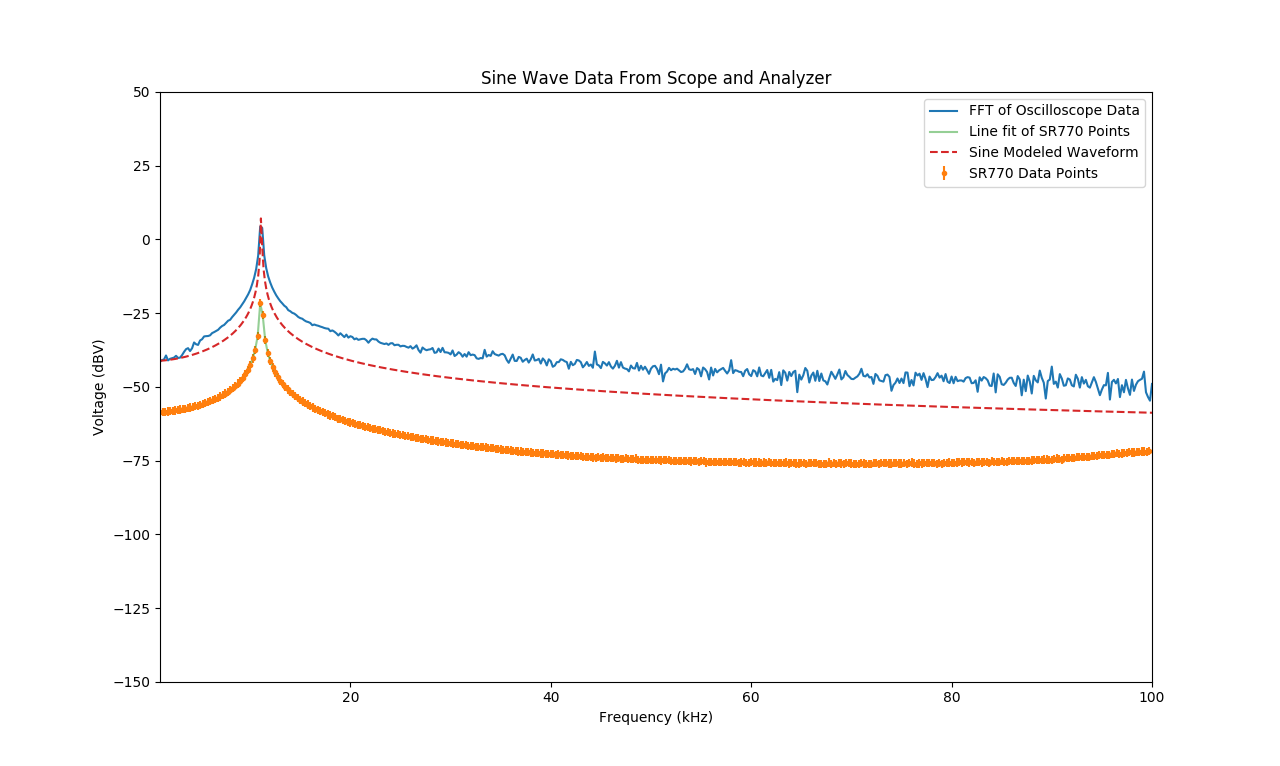
\includegraphics[width=10cm, height=6cm]{figures/figure7.png}
        \caption{Adding a theoretical model to Figure 6}
        \label{fig:fig7}
\end{tcolorbox}
\end{minipage}
\end{figure}

I'm not going to walk though the entire process for the square and triangle
waves; however, here are the final plots that we produced:

\begin{figure}[H]
    \centering
\begin{minipage}{11cm}
\begin{tcolorbox}
        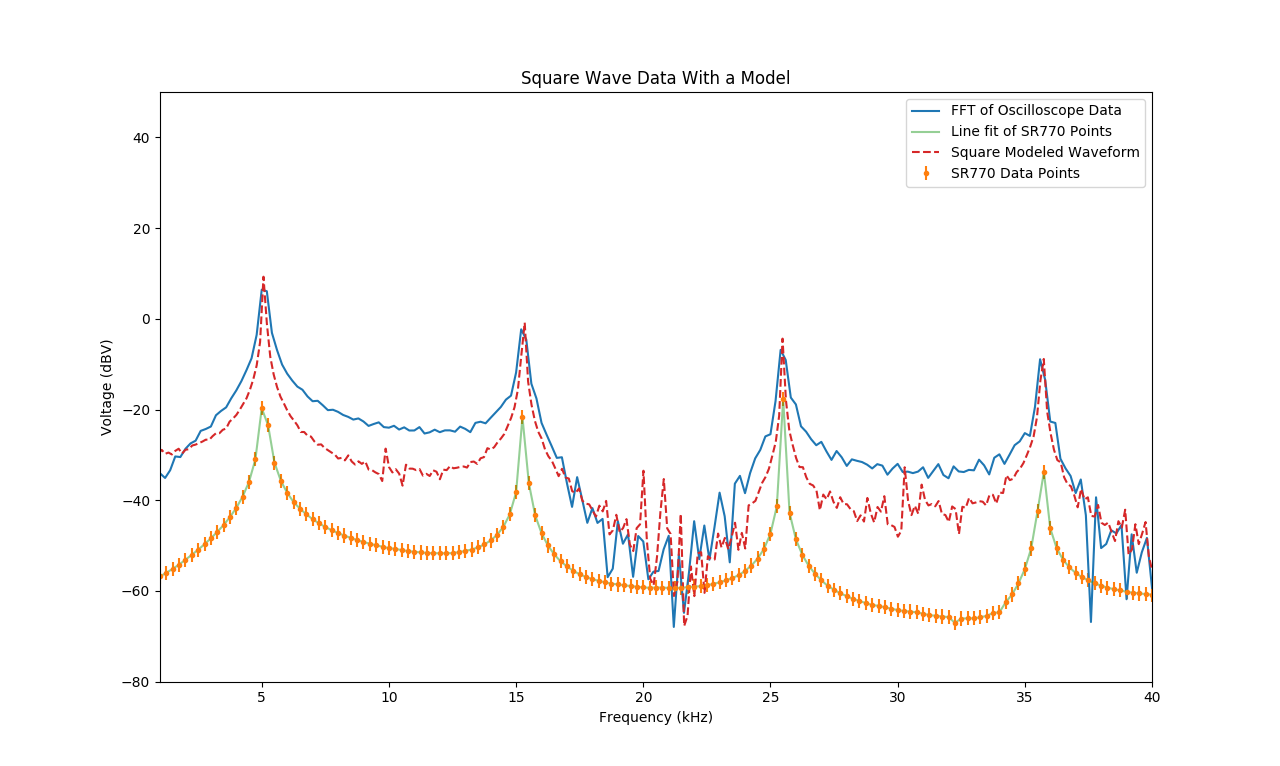
\includegraphics[width=10cm, height=6cm]{figures/figure8.png}
        \caption{Square wave data (including a model)}
        \label{fig:fig8}
\end{tcolorbox}
\end{minipage}
\end{figure}

\begin{figure}[H]
    \centering
\begin{minipage}{11cm}
\begin{tcolorbox}
    \centering
        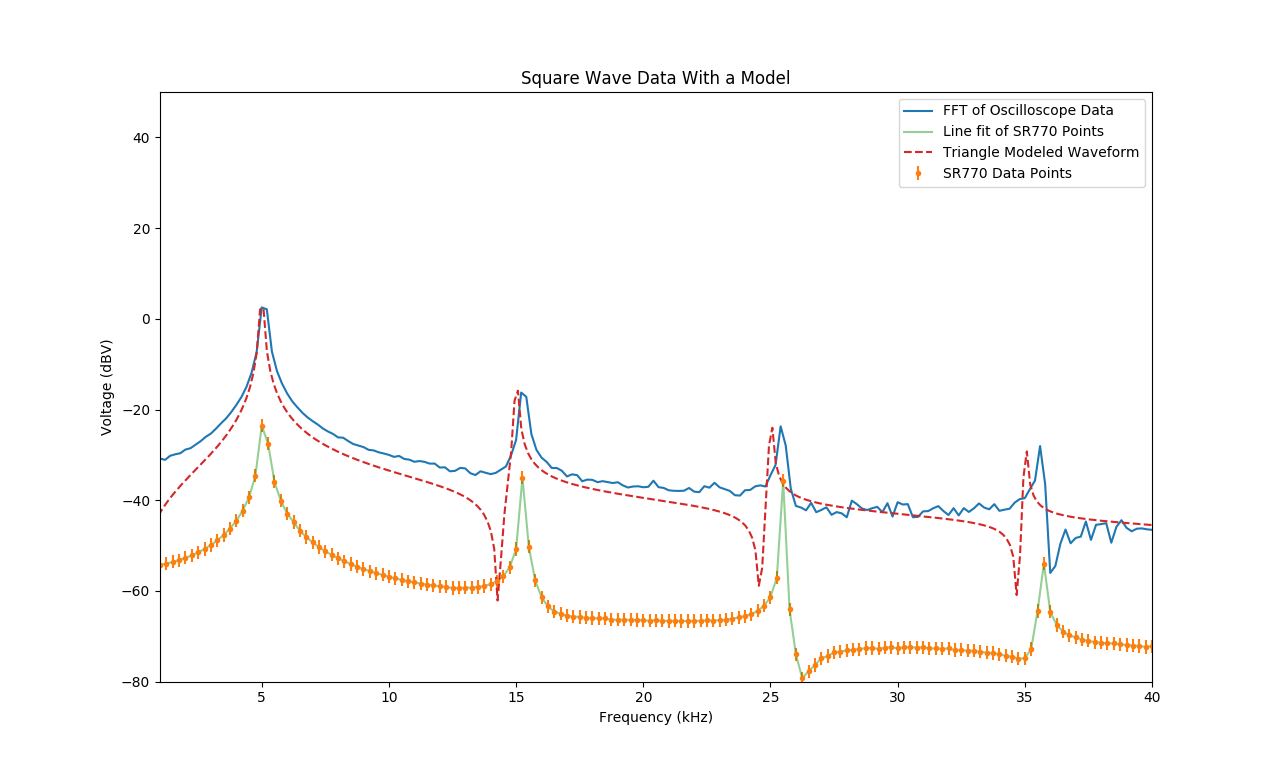
\includegraphics[width=10cm, height=6cm]{figures/figure9.png}
        \caption{Triangle wave data (including a model)}
        \label{fig:fig9}
\end{tcolorbox}
\end{minipage}
\end{figure}

\subsubsection{Summer Module}%
The process for the summer and multiplier modules was extremely similar. The
only difference is that we fed the input signal from the signal generator
through the ``Addition" module instead of running it directly into the scope.

\begin{figure}[H]
    \centering
\begin{minipage}{11cm}
\begin{tcolorbox}
    \centering
        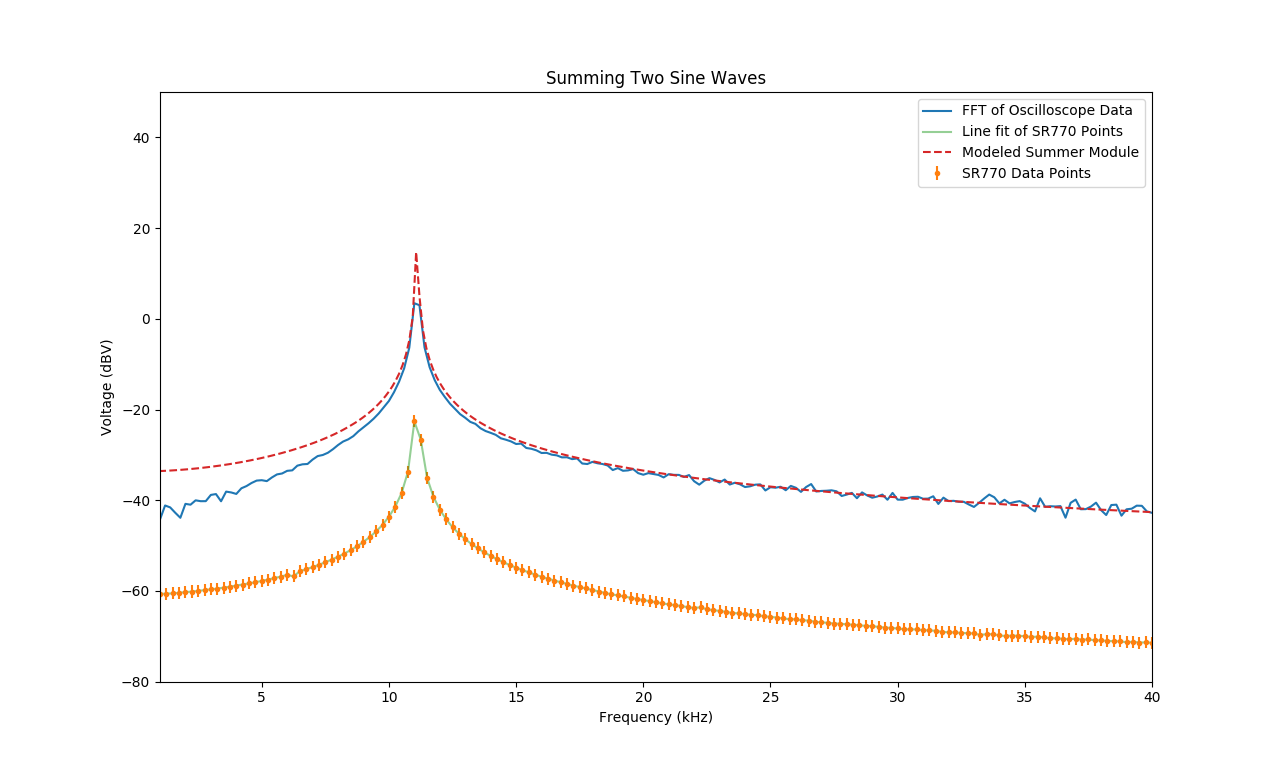
\includegraphics[width=10cm, height=6cm]{figures/figure10.png}
        \caption{Summing two sine waves. Wave A has a frequency of 11.097 kHz
        and peak-to-peak amplitude of 5V. Wave B is 1V at 11.097 kHz.}
        \label{fig:fig10}
\end{tcolorbox}
\end{minipage}
\end{figure}

We noticed that you cannot resolve two peaks when the frequencies are close
together. For example, if we increase the frequency of the second wave to
11.597 kHz, then you can't quite see the second peak on the SR770. You can
actually resolve it by transforming the scope data, but this makes sense
because the scope collects roughly 6 times as many data points as the analyzer
does.

\begin{figure}[H]
    \centering
\begin{minipage}{11cm}
\begin{tcolorbox}
    \centering
        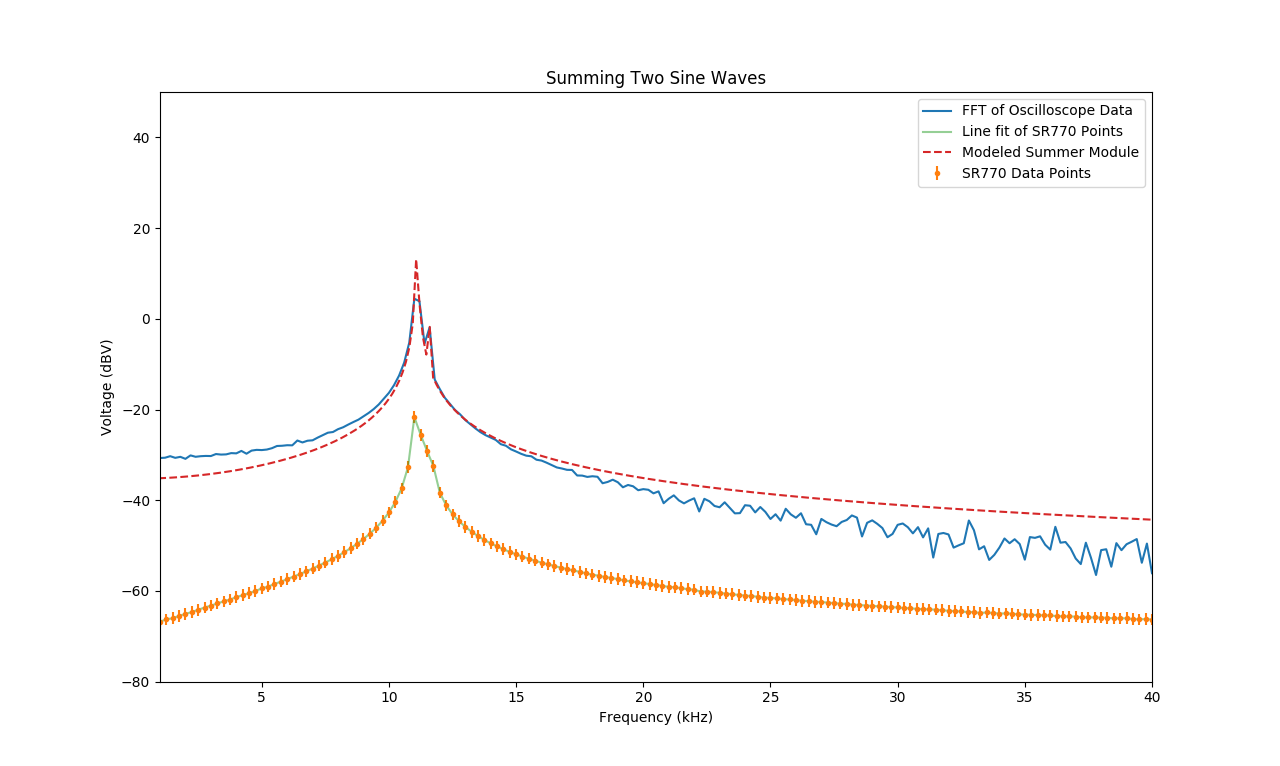
\includegraphics[width=10cm, height=6cm]{figures/figure11.png}
        \caption{Summing two sine waves - SR770 shows a single poorly
        localized peak. Wave A is 5V at 11.097 kHz. Wave B is 1V at 11.597 kHz.}
        \label{fig:fig11}
\end{tcolorbox}
\end{minipage}
\end{figure}

Increasing the frequency of the second wave just a touch more, we are able to
resolve two peaks on the SR770:

\begin{figure}[H]
    \centering
\begin{minipage}{11cm}
\begin{tcolorbox}
    \centering
        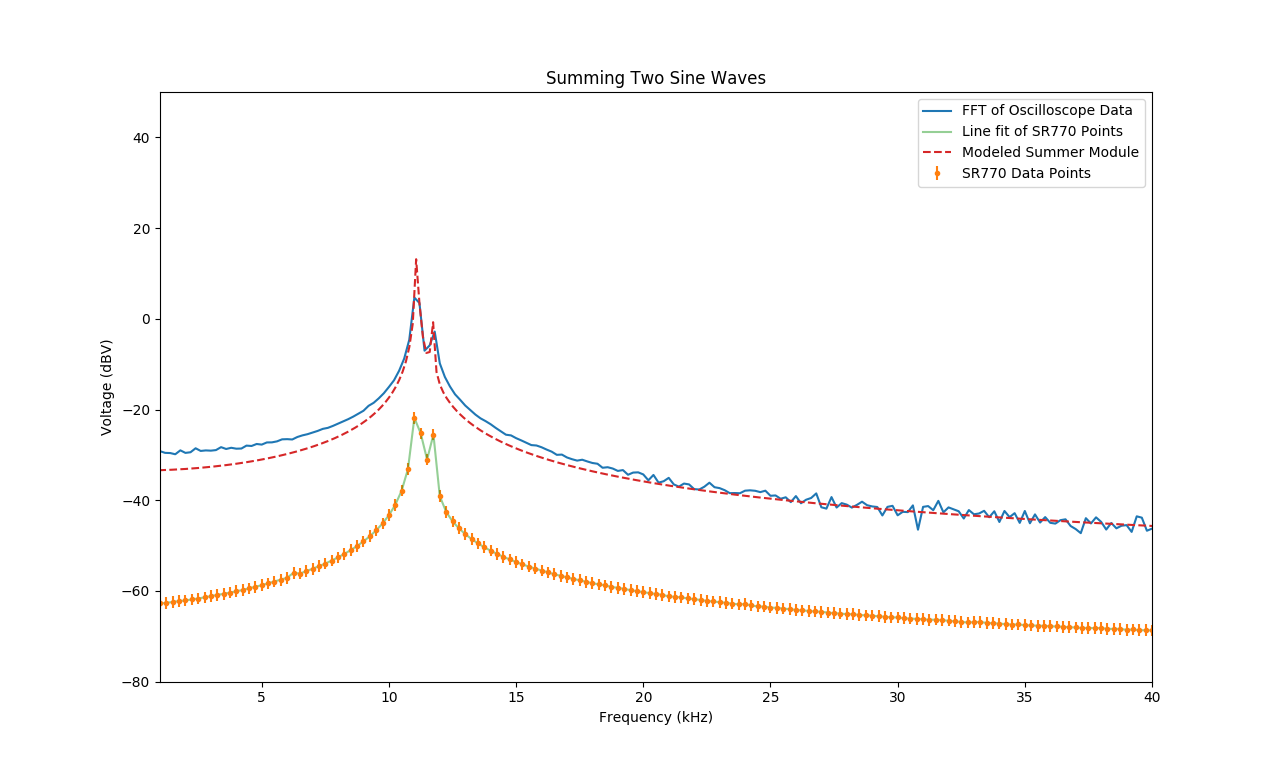
\includegraphics[width=7cm, height=4.5cm]{figures/figure12.png}
        \caption{Summing two sine waves - SR770 shows two peaks.
        Wave A is 5V at 11.097 kHz. Wave B is 1V at 11.697 kHz.}
        \label{fig:fig12}
\end{tcolorbox}
\end{minipage}
\end{figure}

If we separate the frequency substantially, the second peak becomes even more
obvious:

\begin{figure}[H]
    \centering
\begin{minipage}{11cm}
\begin{tcolorbox}
    \centering
        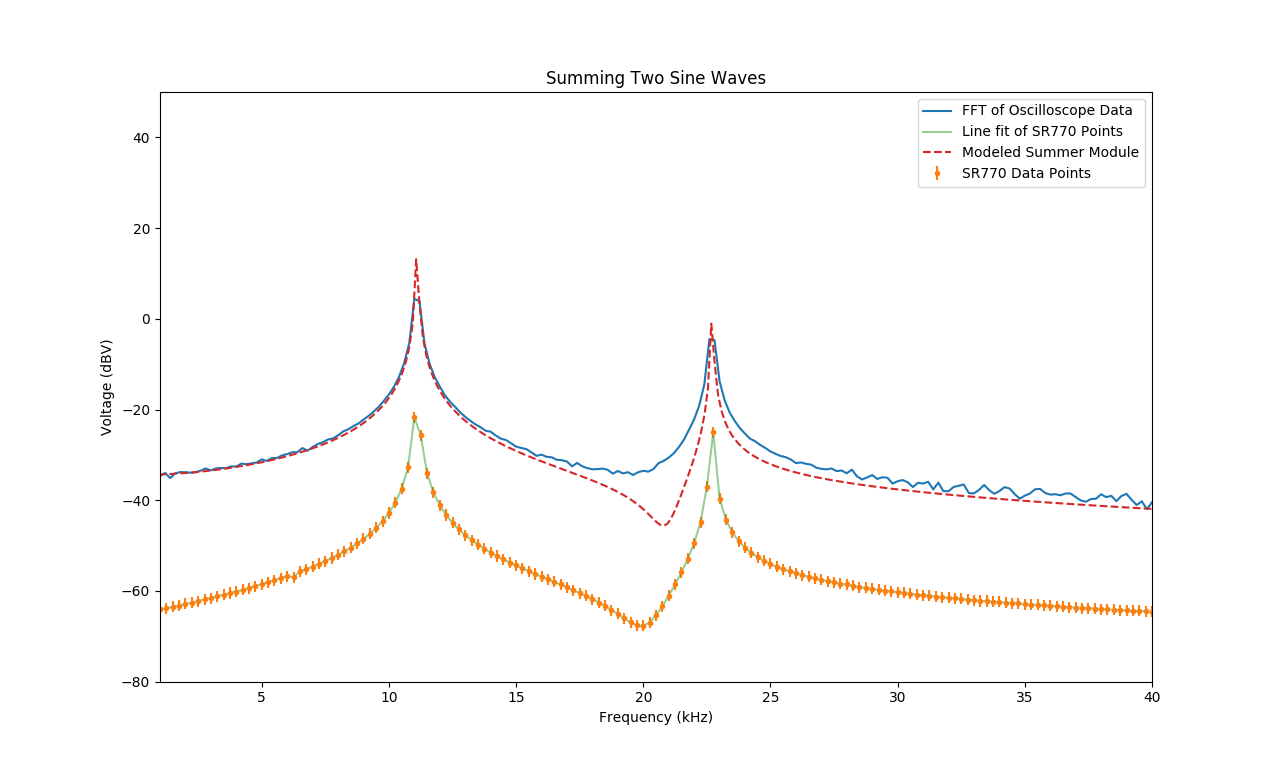
\includegraphics[width=10cm, height=6cm]{figures/figure13.png}
        \caption{Summing two sine waves - two well resolved peaks. Wave A is 5V
        at 11.097 kHz. Wave B is 1V at 22.697 kHz.}
        \label{fig:fig13}
\end{tcolorbox}
\end{minipage}
\end{figure}

\subsubsection{Multiplier Module}%
Moving on to the multiplier module, we see very similar results:

\begin{figure}[H]
    \centering
\begin{minipage}{11cm}
\begin{tcolorbox}
    \centering
        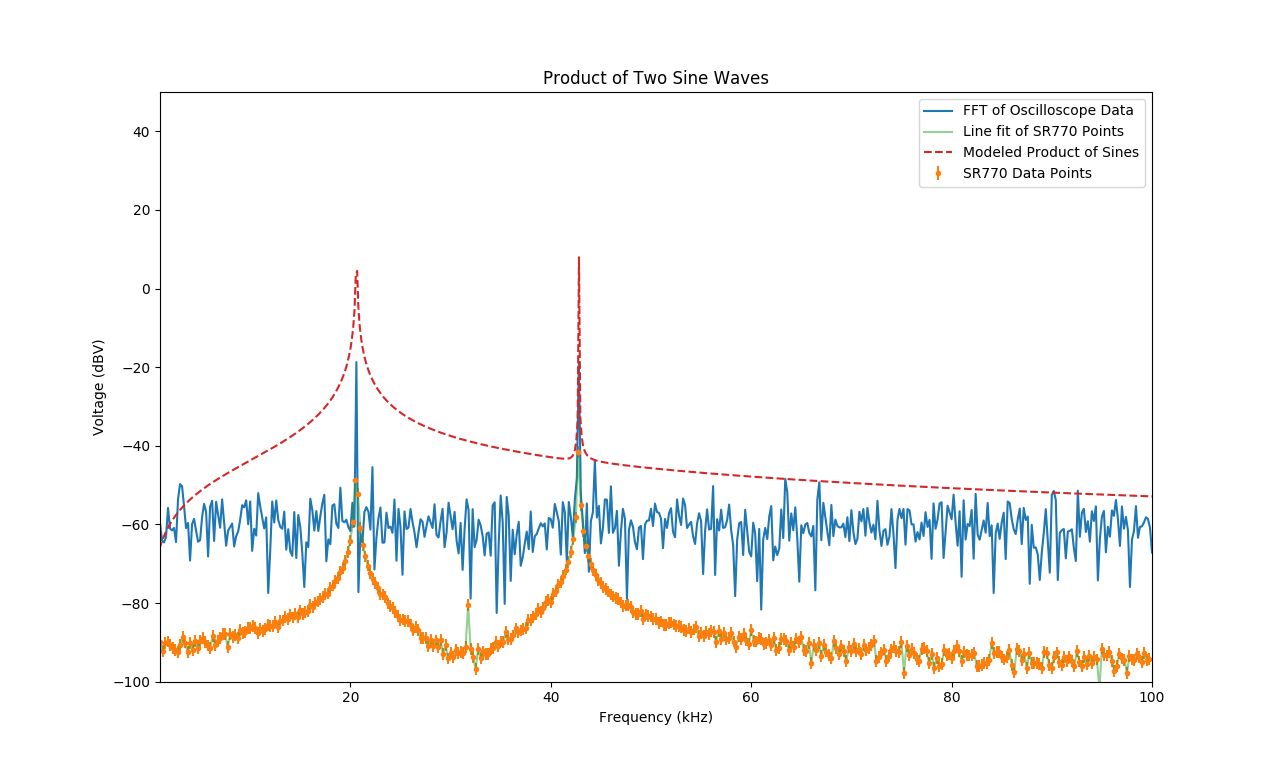
\includegraphics[width=10cm, height=6cm]{figures/figure14.png}
        \caption{Product of two sine waves - two peaks present. Wave A is 5V at
        11.097 kHz. Wave B is 1V at 31.697 kHz.}
        \label{fig:fig14}
\end{tcolorbox}
\end{minipage}
\end{figure}

And setting both input waves to the same frequency:

\begin{figure}[H]
    \centering
\begin{minipage}{11cm}
\begin{tcolorbox}
    \centering
        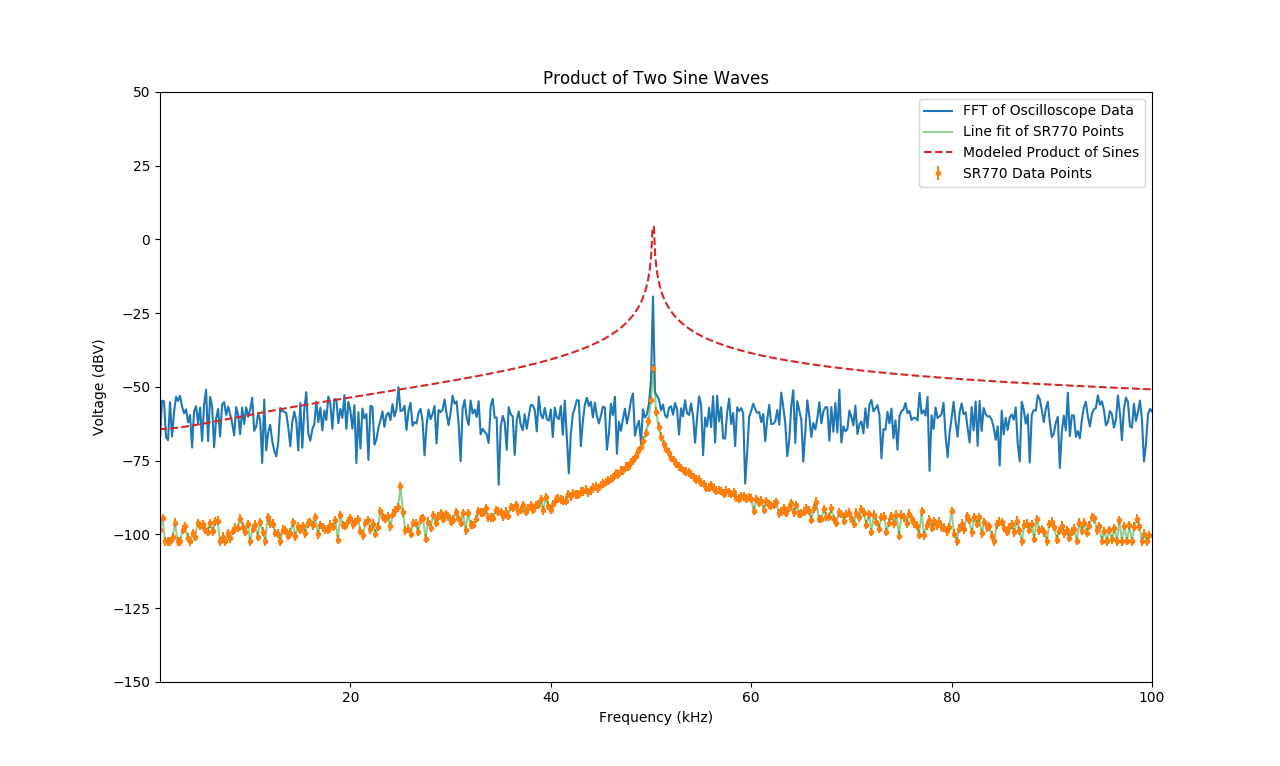
\includegraphics[width=10cm, height=6cm]{figures/figure15.png}
        \caption{Product of two sine waves - single peak present. Wave A is 5V
        at 25.097 kHz. Wave B is 1V at 25.097 kHz}
        \label{fig:fig15}
\end{tcolorbox}
\end{minipage}
\end{figure}


%\pagebreak
\subsubsection{Buried Treasure Module}%
\label{sub:buried_treasure_module}

The final introductory activity required us to use the "Buried Treasure"
module. This module contains an assortment of noise along with a sine wave
whose amplitude is large enough to dominate and appear on the spectrum
analyzer. There are three different treasures -- treasure A, treasure B, and
treasure C. We were successful in finding the sine waves for A and B. We opted
to skip C because of time constraints. 

\begin{figure}[H]
    \centering
\begin{minipage}{11cm}
\begin{tcolorbox}
    \centering
        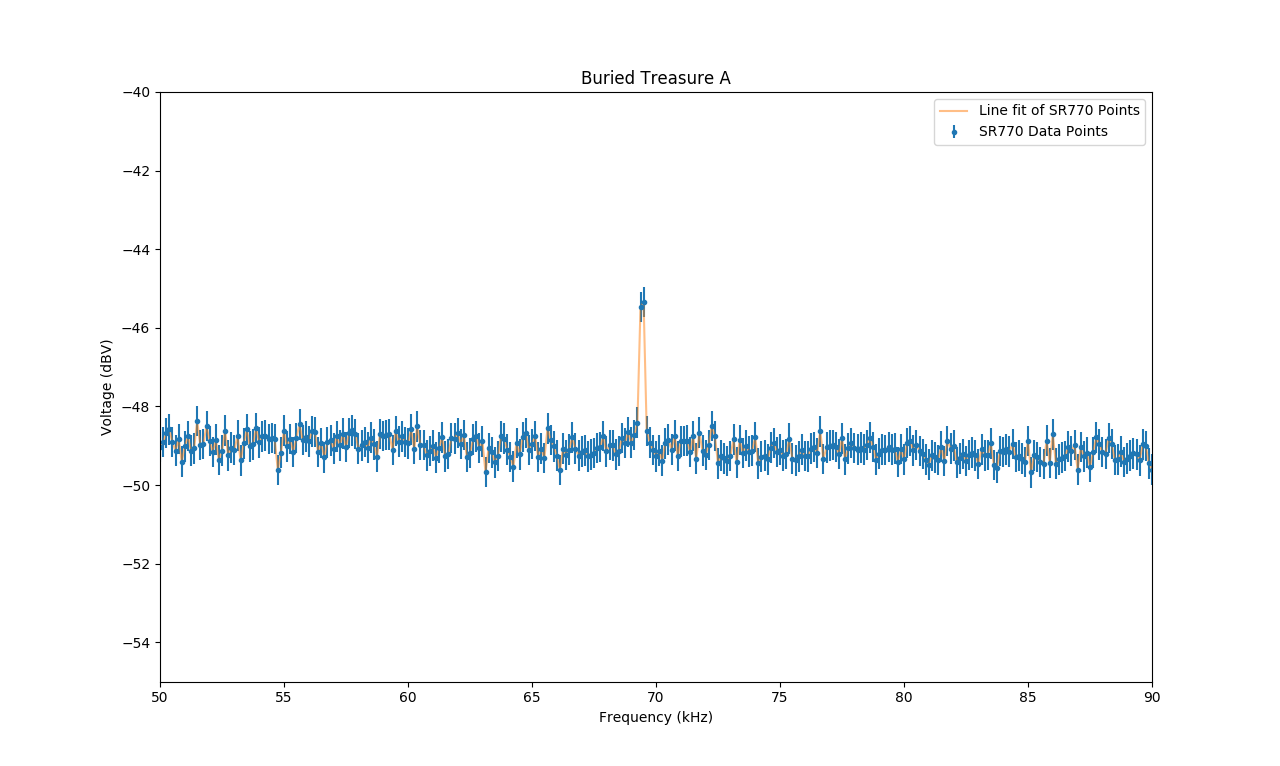
\includegraphics[width=8cm, height=5cm]{figures/figure16.png}
        \caption{Buried treasure 'A' hides a sine wave of approximately 70 kHz}
        \label{fig:fig16}
\end{tcolorbox}
\end{minipage}
\end{figure}

\begin{figure}[H]
    \centering
\begin{minipage}{11cm}
\begin{tcolorbox}
    \centering
        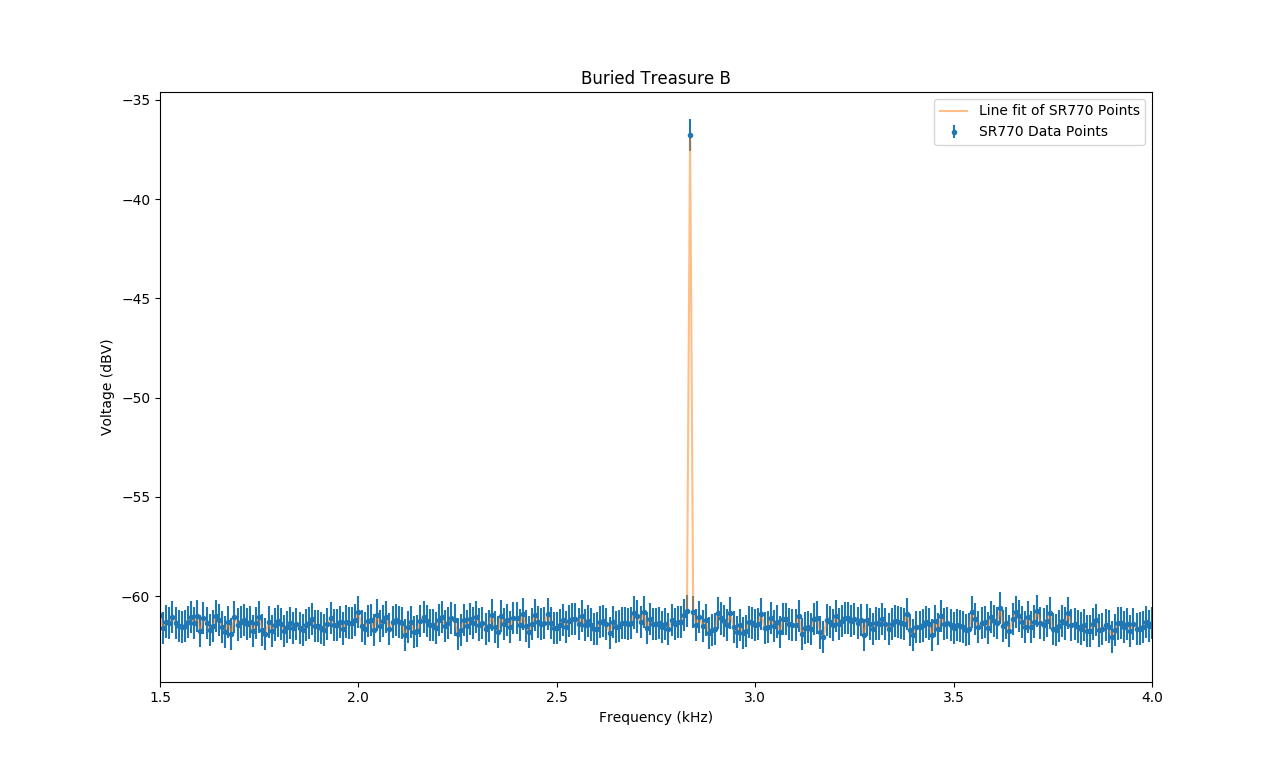
\includegraphics[width=8cm, height=5cm]{figures/figure17.png}
        \caption{Buried Treasure 'B' hides a sine wave of approximately 2.75 kHz}
        \label{fig:fig17}
\end{tcolorbox}
\end{minipage}
\end{figure}

\subsection{LRC Filter}%
\label{sub:lrc_filter}

After completing the introductory exercises, we proceeded to investigate the
LRC circuit. Our goal was to characterize the circuit's response to a variety
of conditions. The circuit's components were all in series to each other and we
measured the $V_{out}$ as the voltage across the capacitor:

\begin{figure}[H]
    \centering
\begin{minipage}{11cm}
\begin{tcolorbox}
    \centering
        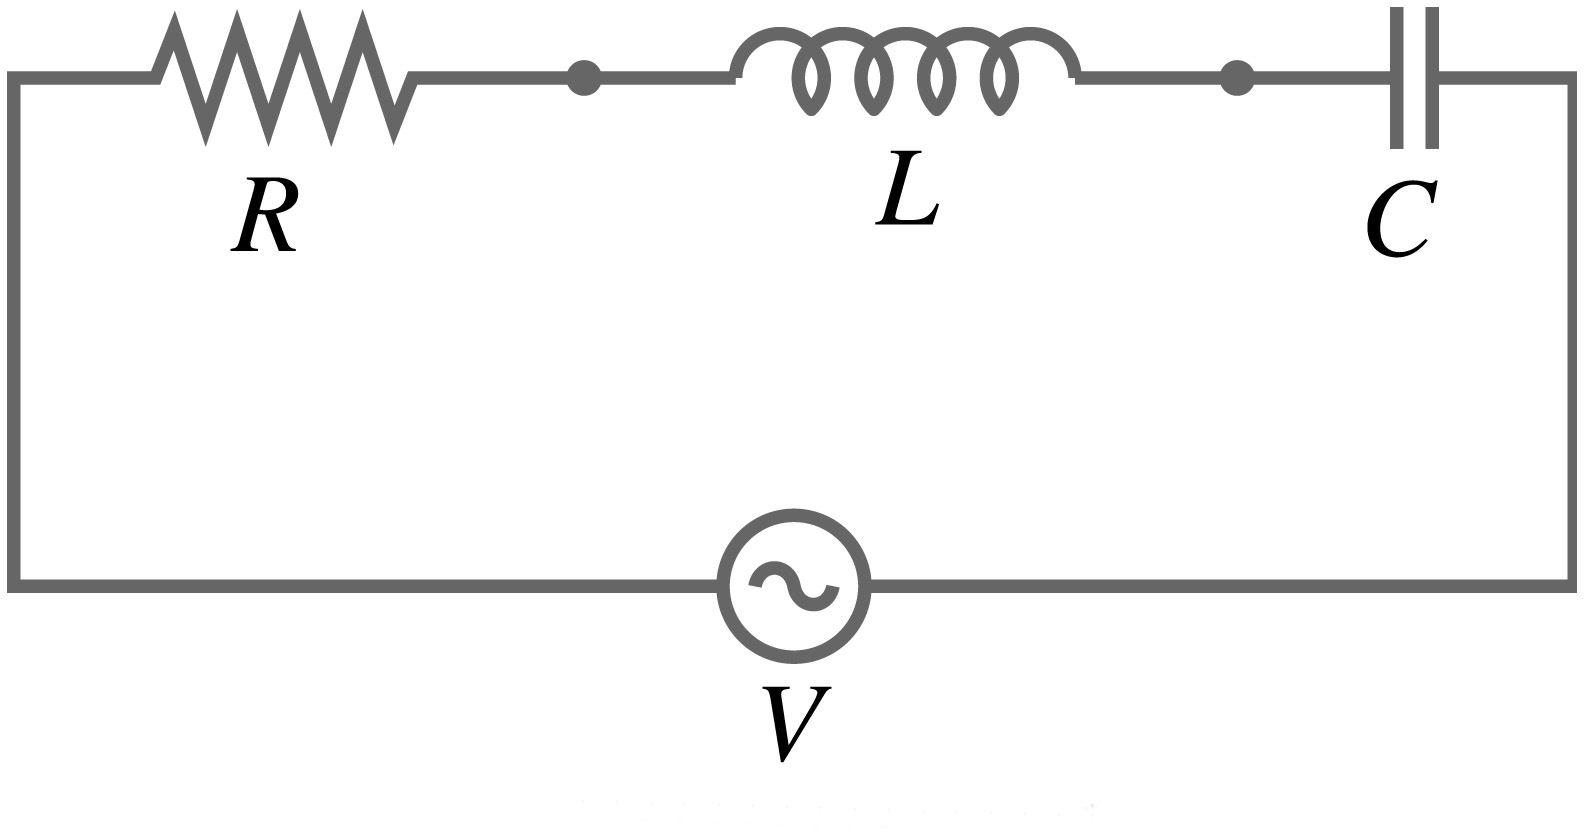
\includegraphics[width=10cm, height=6cm]{figures/figure18.png}
        \caption{LRC circuit diagram with components in series (Image courtesy
        of augustana.edu)}
        \label{fig:fig18}
\end{tcolorbox}
\end{minipage}
\end{figure}

We are provided with (and verify) the values for R, L, and C in this circuit.
This makes it easy to calculate the theoretical fundamental resonant frequency
using

\begin{equation}
    \omega_0 = \frac{1}{\sqrt{LC}}
\end{equation}

Plugging in the values:

\begin{equation*}
    L = 68mH
\end{equation*}

\begin{equation*}
    R = 1000 \Omega
\end{equation*}

\begin{equation*}
    C = 10nF
\end{equation*}

We expect this circuit to have a natural frequency of 6103.313 Hz. In the
coming sections, I will show that this is indeed the case. 

The theoretical models in this section got interesting. In general, the
transfer function of a circuit is a complex function that takes the form

\begin{equation}
    \tilde{H}(\omega) = \frac{\tilde{V}_{out}}{\tilde{V}_{in}}
\end{equation}

In class, we derived $\tilde{H}(\omega)$ for this particular circuit

\begin{equation}
    \tilde{H}_{LRC}(\omega) = \frac{1}{1 - \omega^2 L C + i \omega R C}
\end{equation}

This gives a magnitude of

\begin{equation}
    \|\tilde{H}_{LRC}(\omega)\| = \sqrt{\frac{1}{ \omega^2 R^2 C^2 + (1 -  \omega^ 2 L C)^2}}
\end{equation}

And a phase of 
\begin{equation}
    \phi = -\arctan{\frac{Im}{Re}} = -\arctan{\frac{\omega R C}{1 - \omega^2 L R}}
\end{equation}

Both of these equations will be invaluable in the following sections.

\subsubsection{Single Frequency Drive}%
\label{ssub:single_frequency_drive}

As before, the first step in understanding and characterizing the circuit is to
pass a single frequency through it and plot the results. For the remainder of
the lab, I will not be plotting the oscilloscope data. At this point, it should
be obvious that I understand the process of transforming data between the time
and frequency domains. 

When we pass a single frequency sine wave through the LRC, we find that there
is a resonance at the input's frequency regardless of its value. For example,
when we pass through a sine wave of 12 kHz, the output looks like this:

\begin{figure}[H]
    \centering
\begin{minipage}{11cm}
\begin{tcolorbox}
    \centering
        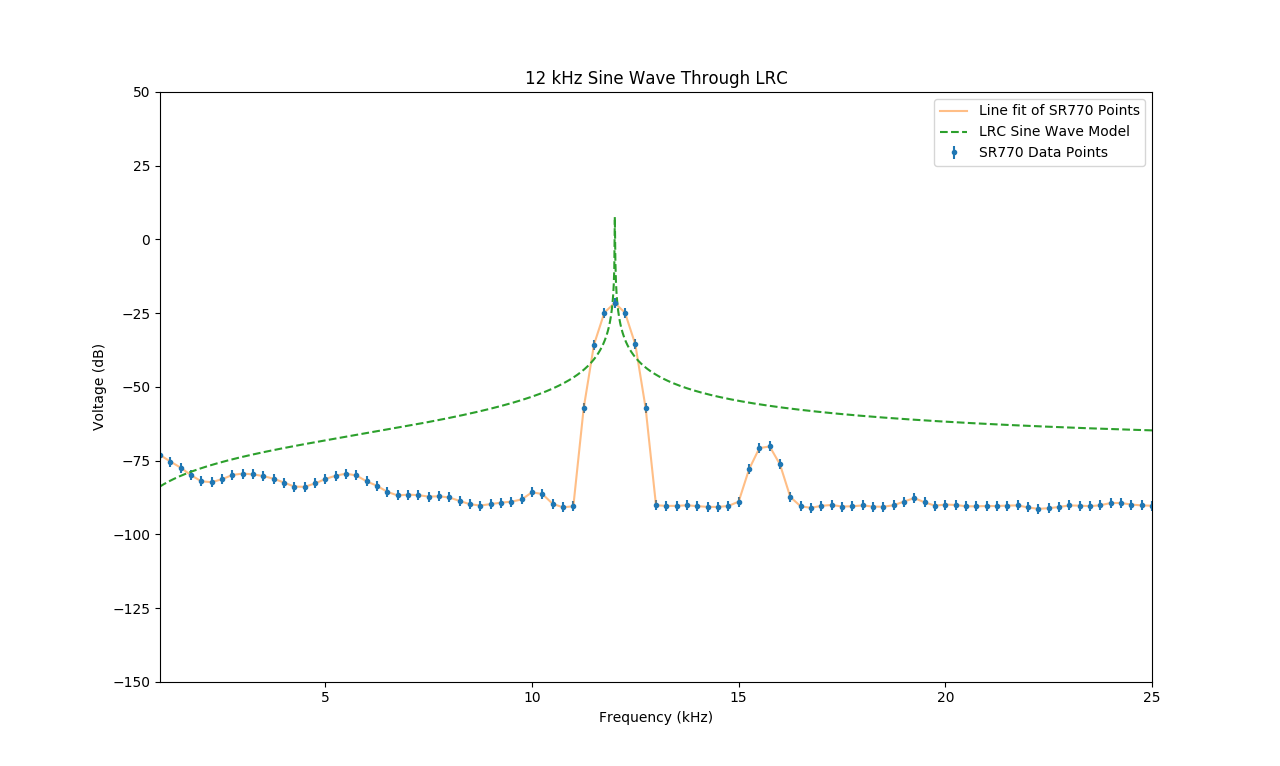
\includegraphics[width=9cm, height=5.5cm]{figures/figure20.png}
        \caption{LRC circuit response to a single frequency sine wave with a
        frequency of 12 kHz}
        \label{fig:fig20}
\end{tcolorbox}
\end{minipage}
\end{figure}

The lab manual makes a point to note that this behavior is unique to single
frequency sines. If we were to pass a single frequency square wave with a
frequency of 12 kHz through the circuit, the output would not necessarily have
a peak at 12 kHz. Just to be thorough, here is a plot of the circuit's response
to an 18 kHz sine wave:

\begin{figure}[H]
    \centering
\begin{minipage}{11cm}
\begin{tcolorbox}
    \centering
        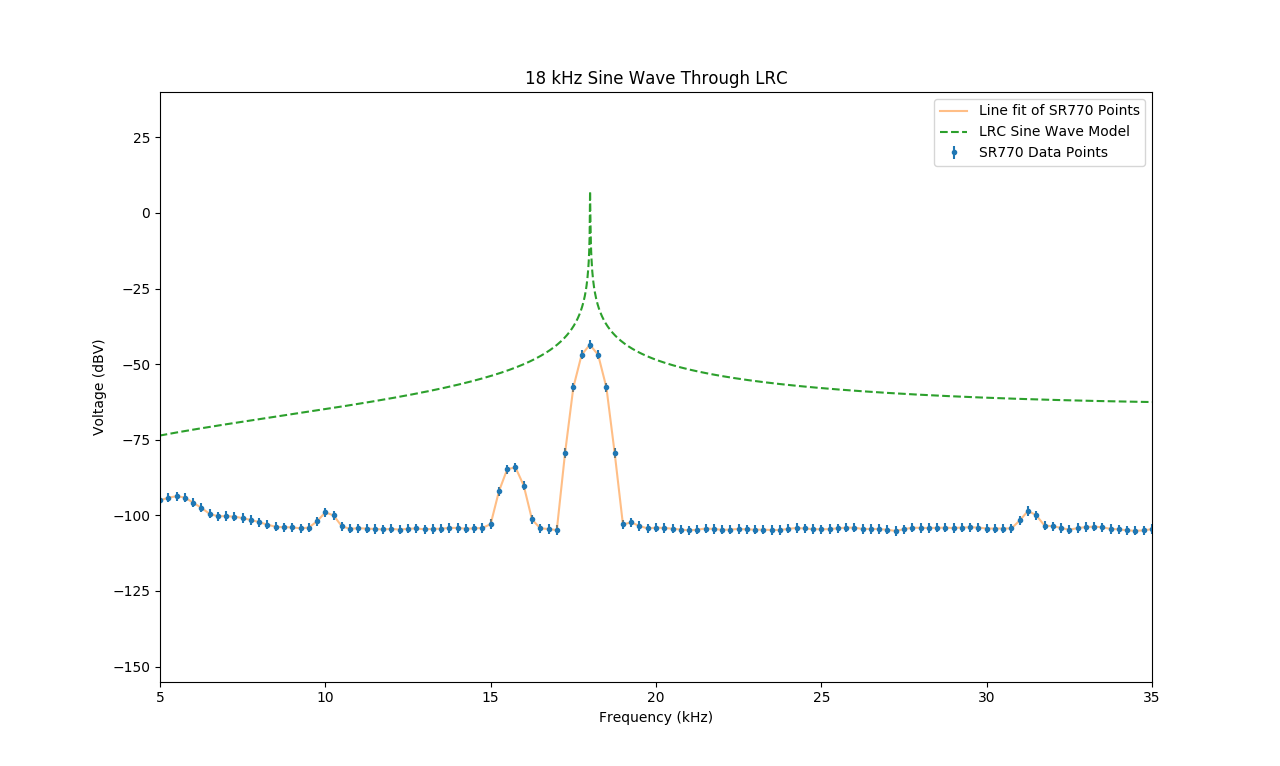
\includegraphics[width=10cm, height=6cm]{figures/figure21.png}
        \caption{LRC circuit response to a single frequency 18 kHz sine wave}
        \label{fig:fig21}
\end{tcolorbox}
\end{minipage}
\end{figure}

\subsubsection{Noise Drive}%
\label{ssub:noise_drive}

After driving the LRC with several single frequency inputs -- it was time to
investigate the circuit's response to noise. Typical white noise consists of a
Gaussian distribution of sine waves over a range of frequencies. We used the
``noise" setting on the buried treasure module because its frequencies were low
enough to avoid causing hardware issues.

Unfortunately, we did not record the array of input voltages. This makes it
impossible to recover the units for the data collected. We can't get the
amplitude parameter from experimental data. So, when we plot the model, we find
that the frequency of the peak lines up perfectly while the amplitudes do not
match at all.

\begin{figure}[H]
    \centering
\begin{minipage}{11cm}
\begin{tcolorbox}
    \centering
        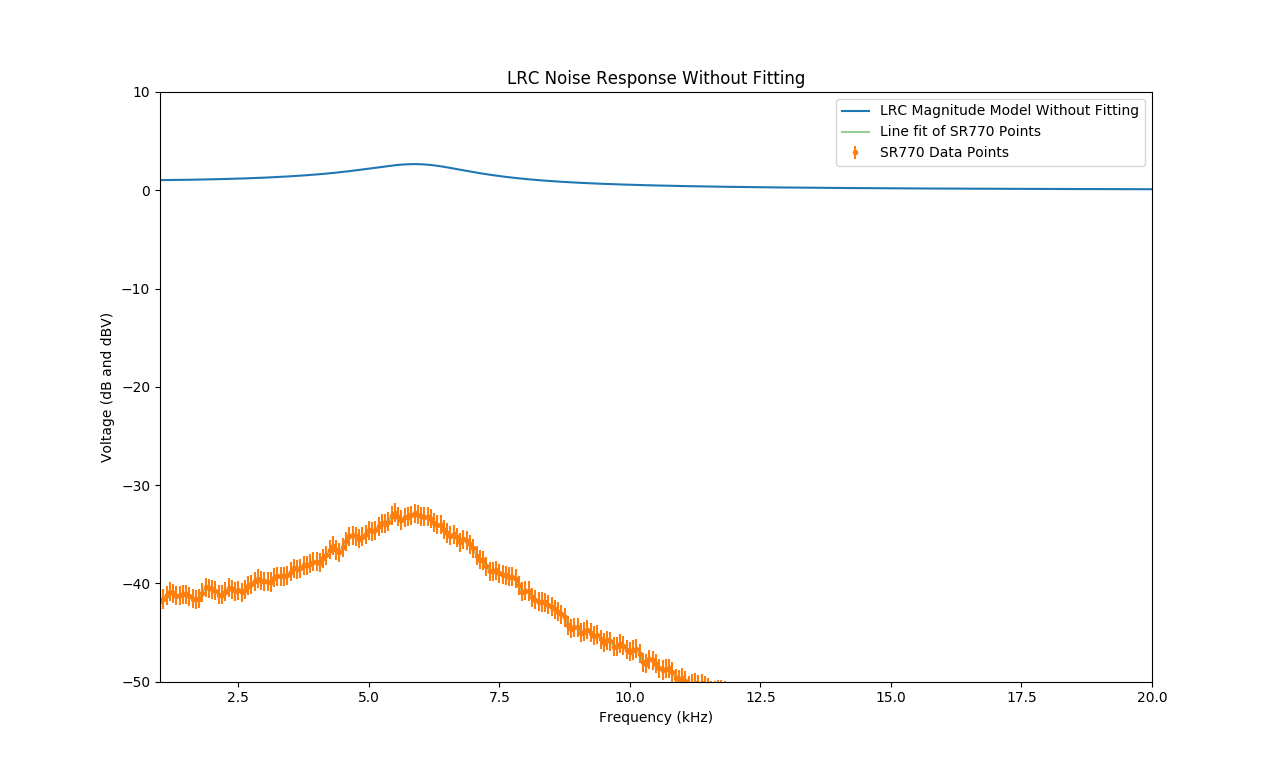
\includegraphics[width=10cm, height=6cm]{figures/figure22.png}
        \caption{LRC circuit's response to a noise drive without matching
        amplitudes}
        \label{fig:fig22}
\end{tcolorbox}
\end{minipage}
\end{figure}

Fortunately, we can use the curve\_fit function in order to artificially
recover the parameters. In other words, we can find the values for amplitude,
capacitance, resistance, and inductance that best fit the theoretical model to
the data. Once we do this, the plot gets much prettier.

\begin{figure}[H]
    \centering
\begin{minipage}{11cm}
\begin{tcolorbox}
    \centering
        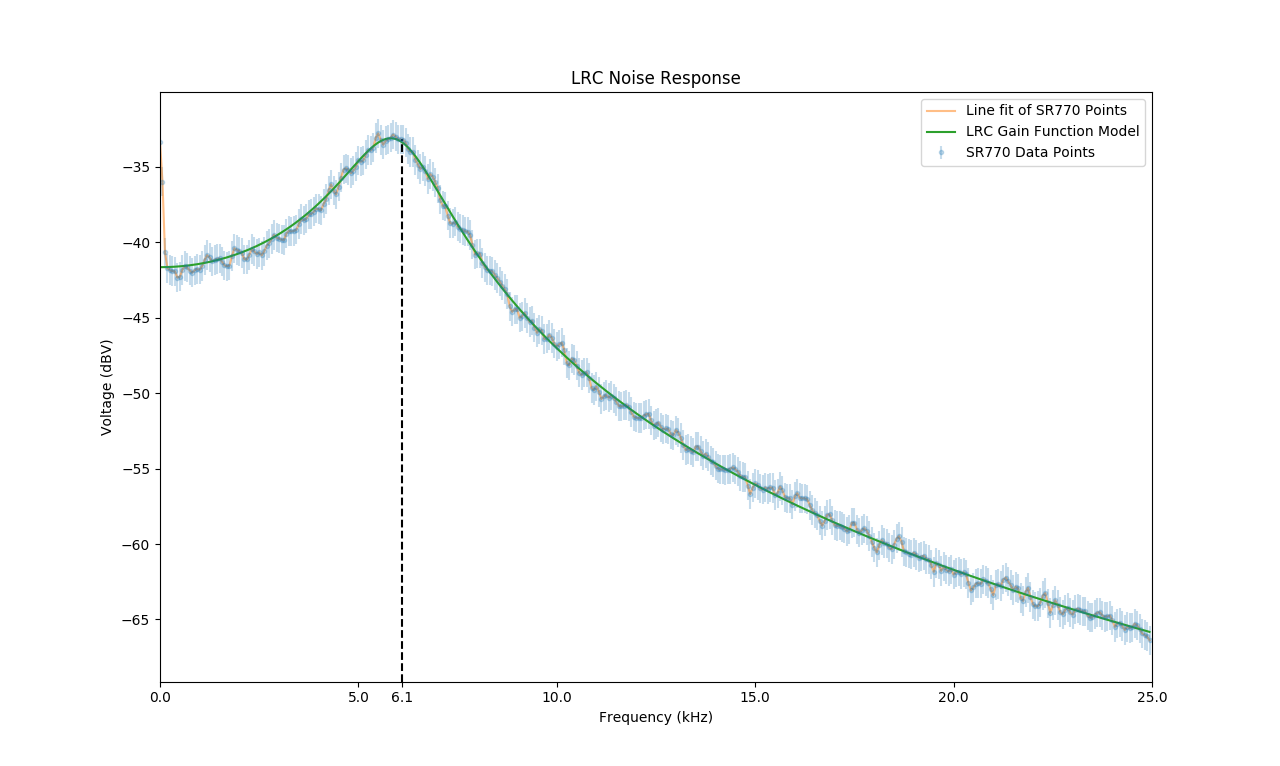
\includegraphics[width=10cm, height=6cm]{figures/figure23.png}
        \caption{LRC circuit response to a noise drive}
        \label{fig:fig22}
\end{tcolorbox}
\end{minipage}
\end{figure}

During lecture, we predicted the peak of the response to be at a frequency
slightly beneath the natural frequency. Experimentally, we can see that this is
in fact the case!

\subsubsection{Chirp Drive}%
\label{ssub:chirp_drive}

The results of driving the LRC with a chirp are extremely similar to those of
driving it with noise -- except that it is possible to recover the complex
phase information.

\begin{figure}[H]
    \centering
\begin{minipage}{11cm}
\begin{tcolorbox}
    \centering
        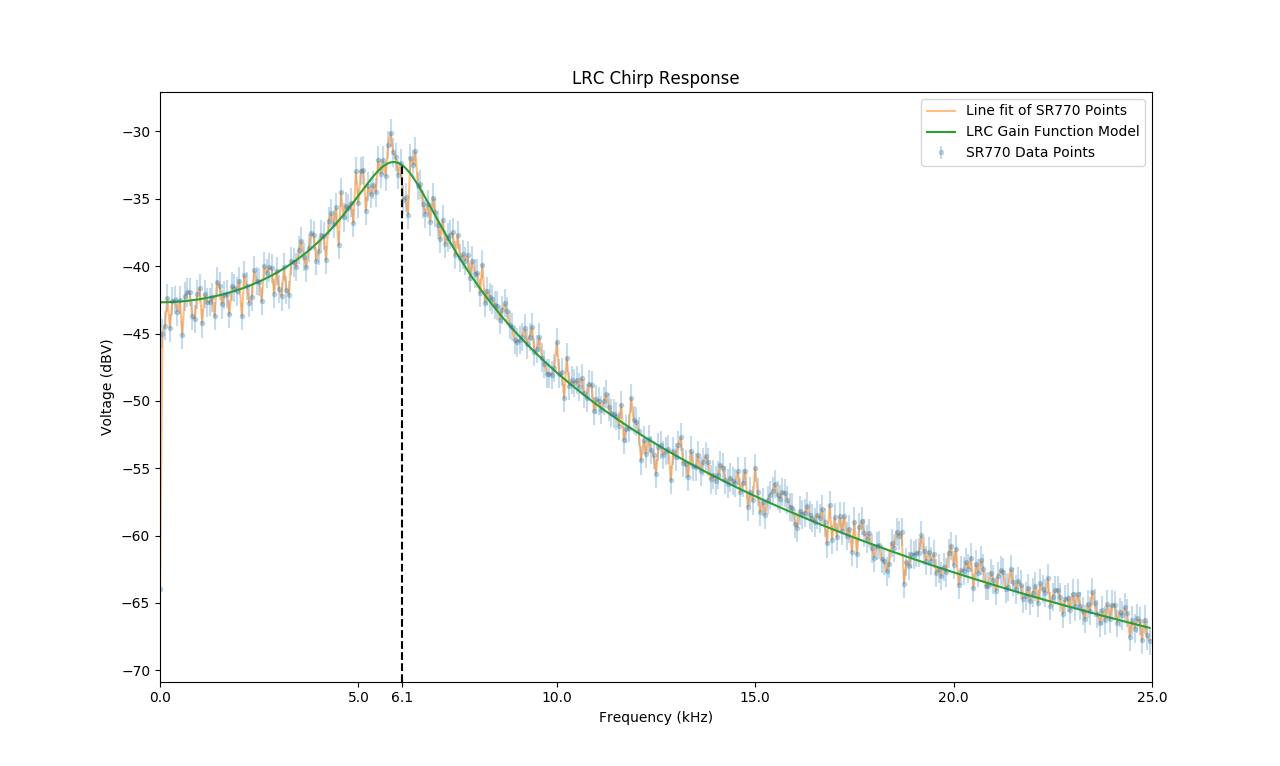
\includegraphics[width=10cm, height=6cm]{figures/figure24.png}
        \caption{LRC circuit response to chirp drive}
        \label{fig:fig24}
\end{tcolorbox}
\end{minipage}
\end{figure}

Unfortunately, all of the groups had some pretty serious issues collecting
phase data. For us, it displayed correctly on the screen of the SR770, but then
the data set came out awful! We collected the data twice and were still unable
to get anything that looked correct. For the sake of completeness, here is the
phase data that we collected:

\begin{figure}[H]
    \centering
\begin{minipage}{11cm}
\begin{tcolorbox}
    \centering
        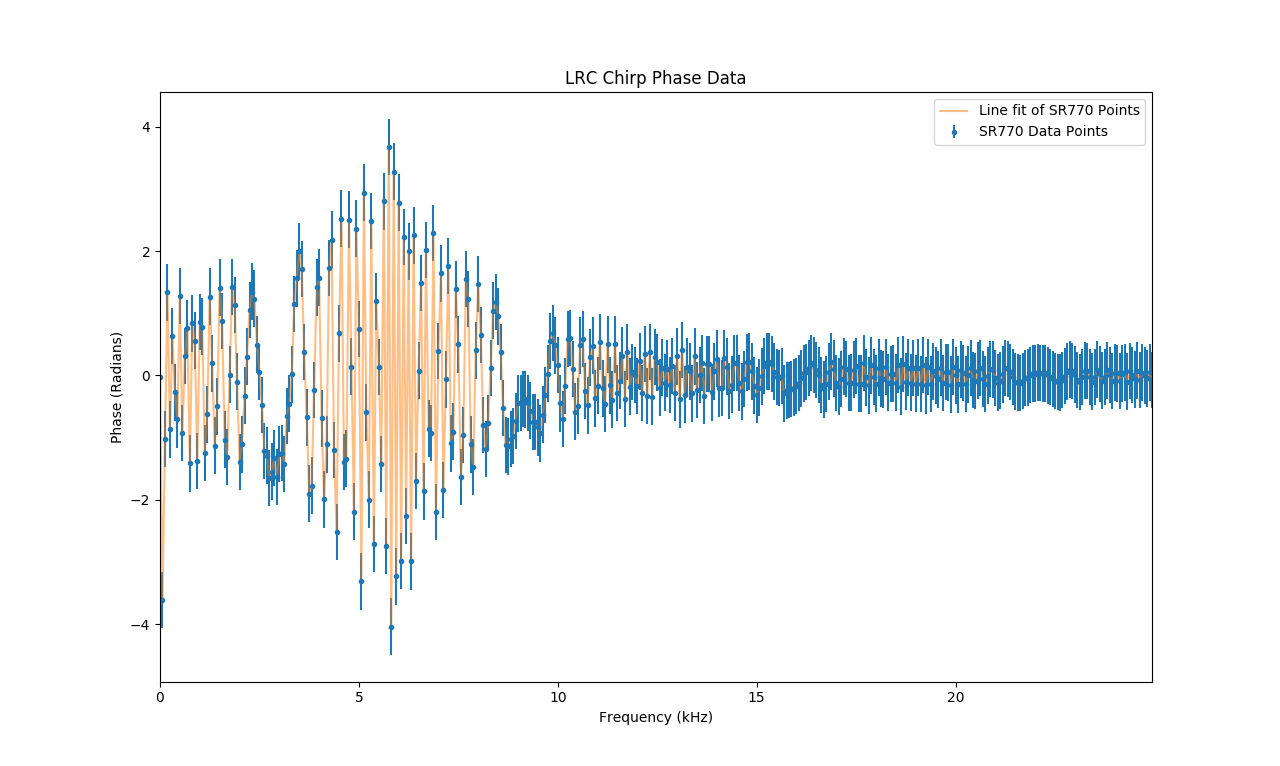
\includegraphics[width=10cm, height=6cm]{figures/figure25.png}
        \caption{LRC phase data (corrupted)}
        \label{fig:fig25}
\end{tcolorbox}
\end{minipage}
\end{figure}

It is easy enough to model the correct phase results using equation (6) and
NumPy's arctan2 method:

\begin{figure}[H]
    \centering
\begin{minipage}{11cm}
\begin{tcolorbox}
    \centering
        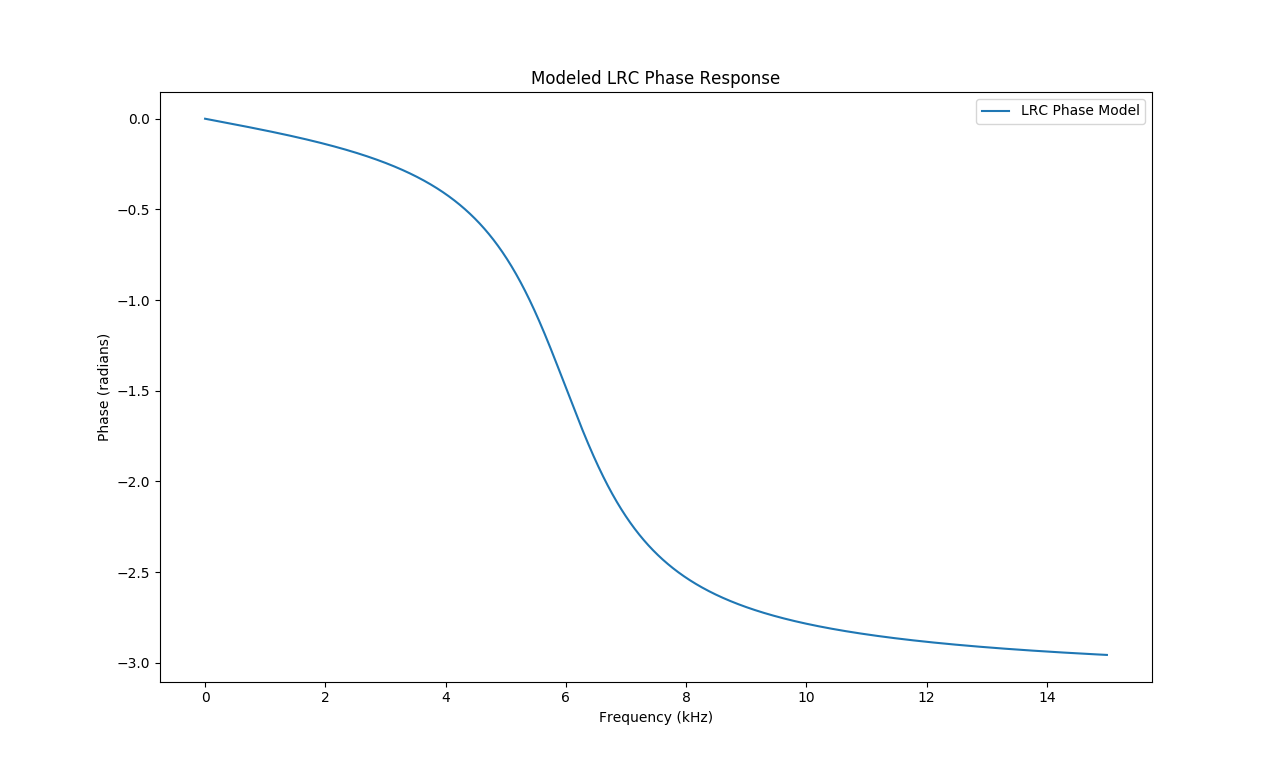
\includegraphics[width=10cm, height=6cm]{figures/figure26.png}
        \caption{LRC phase model (without data)}
        \label{fig:fig26}
\end{tcolorbox}
\end{minipage}
\end{figure}

\subsubsection{Transient Response}%
\label{ssub:transient_response}

The final activity with the LRC circuit involves passing a step function
through the circuit. Plotting the results and model we see that the fundamental
frequency aligns perfectly

\begin{figure}[H]
    \centering
\begin{minipage}{11cm}
\begin{tcolorbox}
    \centering
        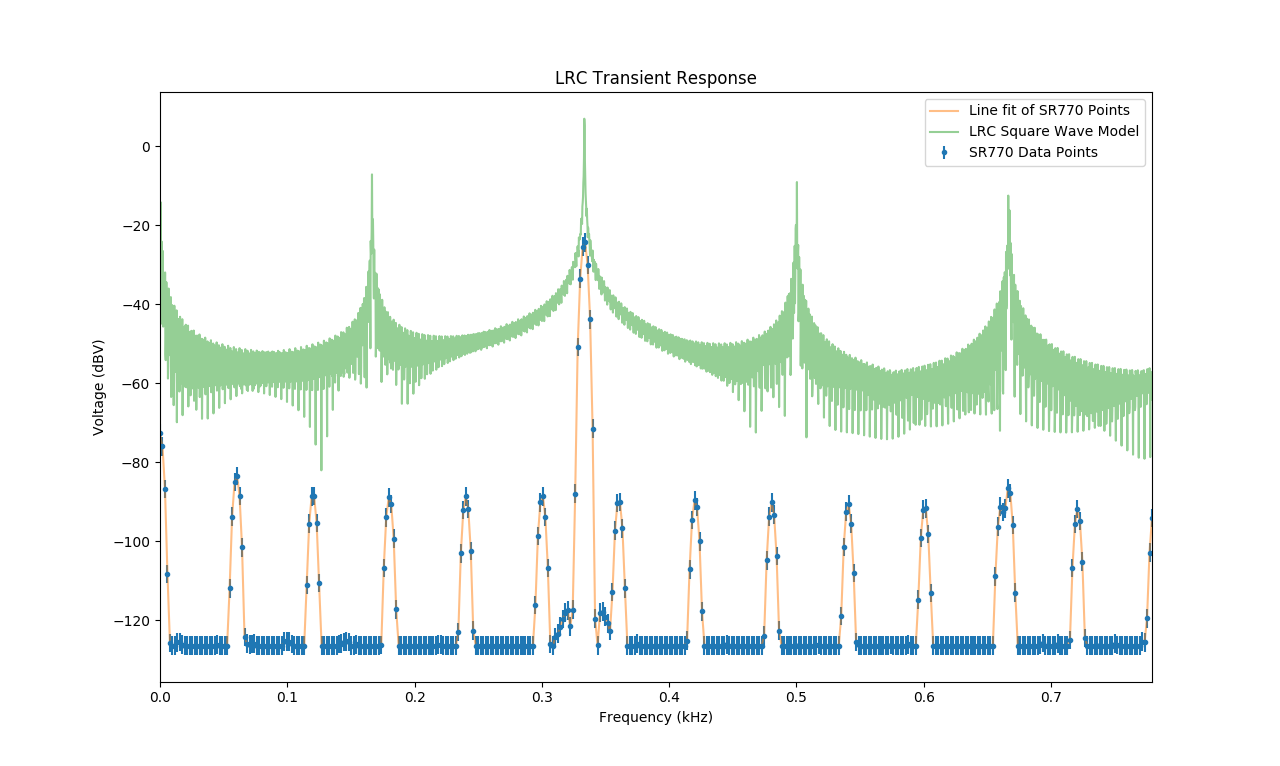
\includegraphics[width=10cm, height=6cm]{figures/figure27.png}
        \caption{LRC transient response data and model}
        \label{fig:fig27}
\end{tcolorbox}
\end{minipage}
\end{figure}

Unfortunately, the harmonics do not match. To me, it looks like there is either
a unit issue, or our model is slightly too naive to catch them.

\subsection{Acoustical Cavity}%
\label{sub:acoustical_cavity}

We did not really discuss the mathematical theory behind the acoustical cavity
in lecture or lab. So, I will exclude it from here as well. The dedicated
reader can easily google resources regarding the resonance of open and closed
cylindrical cavities. Additionally, I will not include theoretical models for
the data. The procedure for this section was almost identical to that of the
preceding section, so I will present the results with a minimal amount of
explanation. Refer to the lab manual or my notebook to rectify any confusion
that occurs.

%Additionally, it seems worth noting that it is possible to excite harmonics
%above the fundamental frequency, but not below. This makes sense because any
%frequency below (IE wavelength above) the fundamental will not physically have
%enough space to resonate
\subsubsection{Single Frequency Drive}%
\label{ssub:single_frequency_drive}

When we use a single frequency sine wave to drive the acoustical cavity, we
find very similar results to those from the LRC circuit. Specifically, we are
able to excite a fundamental harmonic at the driving frequency and `echoes' of
it at higher frequencies

\begin{figure}[H]
    \centering
\begin{minipage}{11cm}
\begin{tcolorbox}
    \centering
        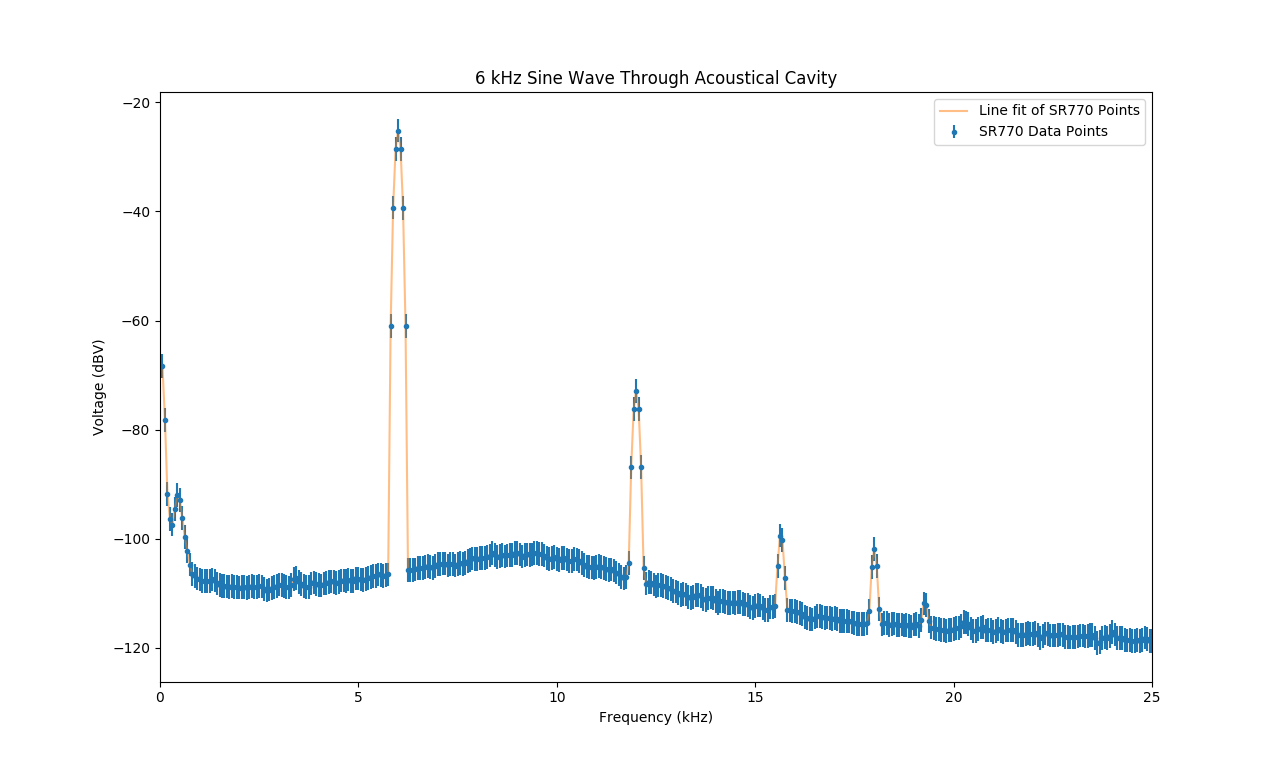
\includegraphics[width=10cm, height=6cm]{figures/figure28.png}
        \caption{Single frequency 6 kHz sine wave resonating through acoustical
        cavity}
        \label{fig:fig28}
\end{tcolorbox}
\end{minipage}
\end{figure}

One interesting tidbit that we noticed and discussed during the lab is that it
is impossible to excite harmonics at frequencies lower than the input
frequency. For example, if we consider passing a 9 kHz sine wave through the
cavity we find that there is no longer a mode at 6 kHz:

\begin{figure}[H]
    \centering
\begin{minipage}{11cm}
\begin{tcolorbox}
    \centering
        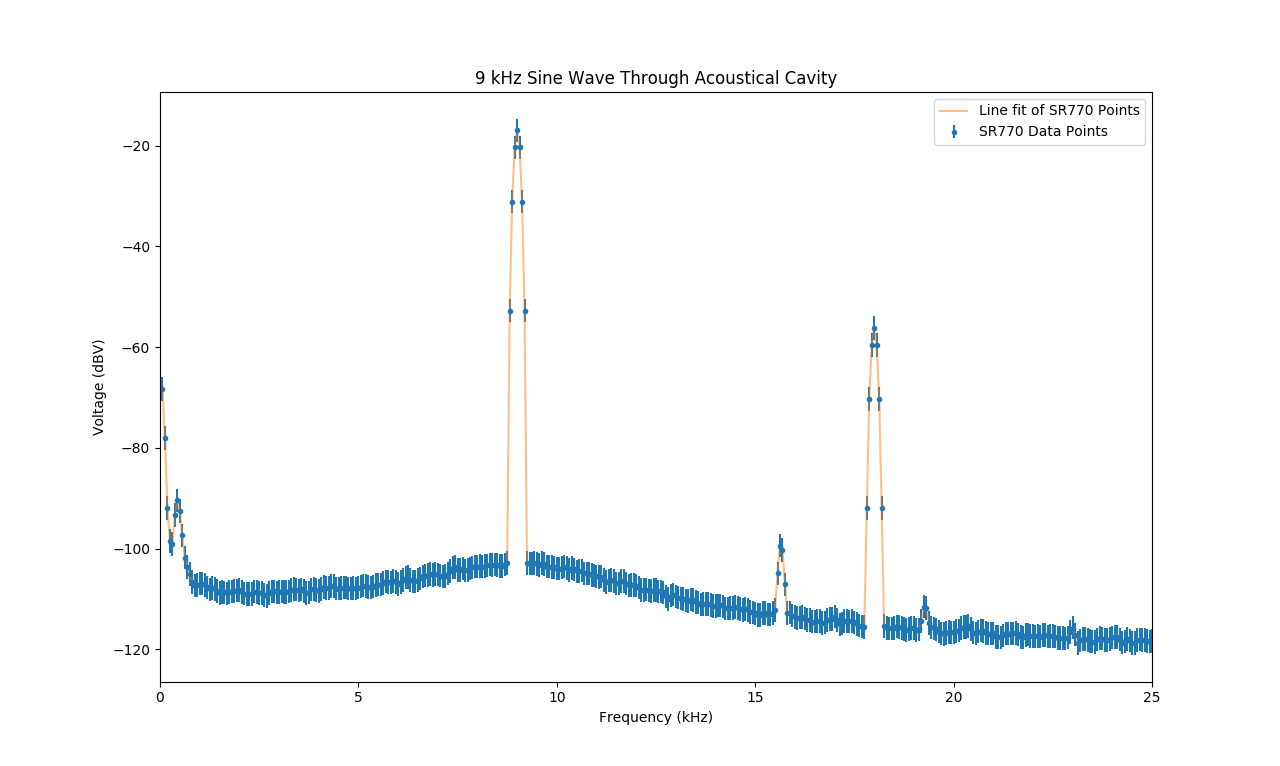
\includegraphics[width=10cm, height=6cm]{figures/figure29.png}
        \caption{Single frequency 9 kHz sine wave resonating through acoustical
        cavity (notice there is no peak at 6 kHz any more)}
        \label{fig:fig29}
\end{tcolorbox}
\end{minipage}
\end{figure}

This is also observable in the 12 kHz data:

\begin{figure}[H]
    \centering
\begin{minipage}{11cm}
\begin{tcolorbox}
    \centering
        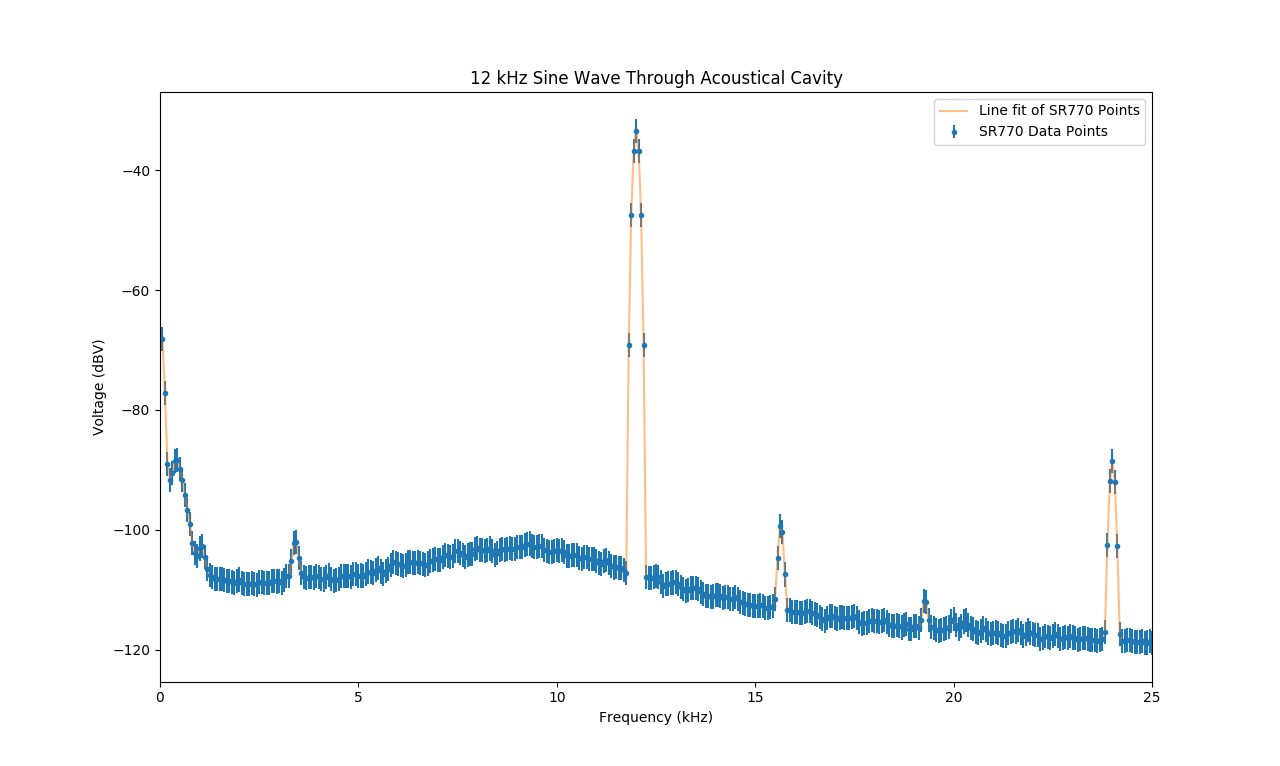
\includegraphics[width=10cm, height=6cm]{figures/figure30.png}
        \caption{Single frequency 12 kHz sine wave resonating through acoustical
        cavity (no longer peaks at 6 or 9 kHz)}
        \label{fig:fig30}
\end{tcolorbox}
\end{minipage}
\end{figure}

\subsubsection{Noise Drive}%
\label{ssub:noise_drive}

The next thing we did was drive the acoustical cavity using noise generated by
the buried treasure module. Unfortunately, it seems as though our data from
this section may also have gotten corrupted somehow. The output that we
produced during lab had quite a few modes that began at the fundamental
frequency and increased (although they were not perfectly even). The analyzer
data file that we saved just looks like noise. 

\begin{figure}[H]
    \centering
\begin{minipage}{11cm}
\begin{tcolorbox}
    \centering
        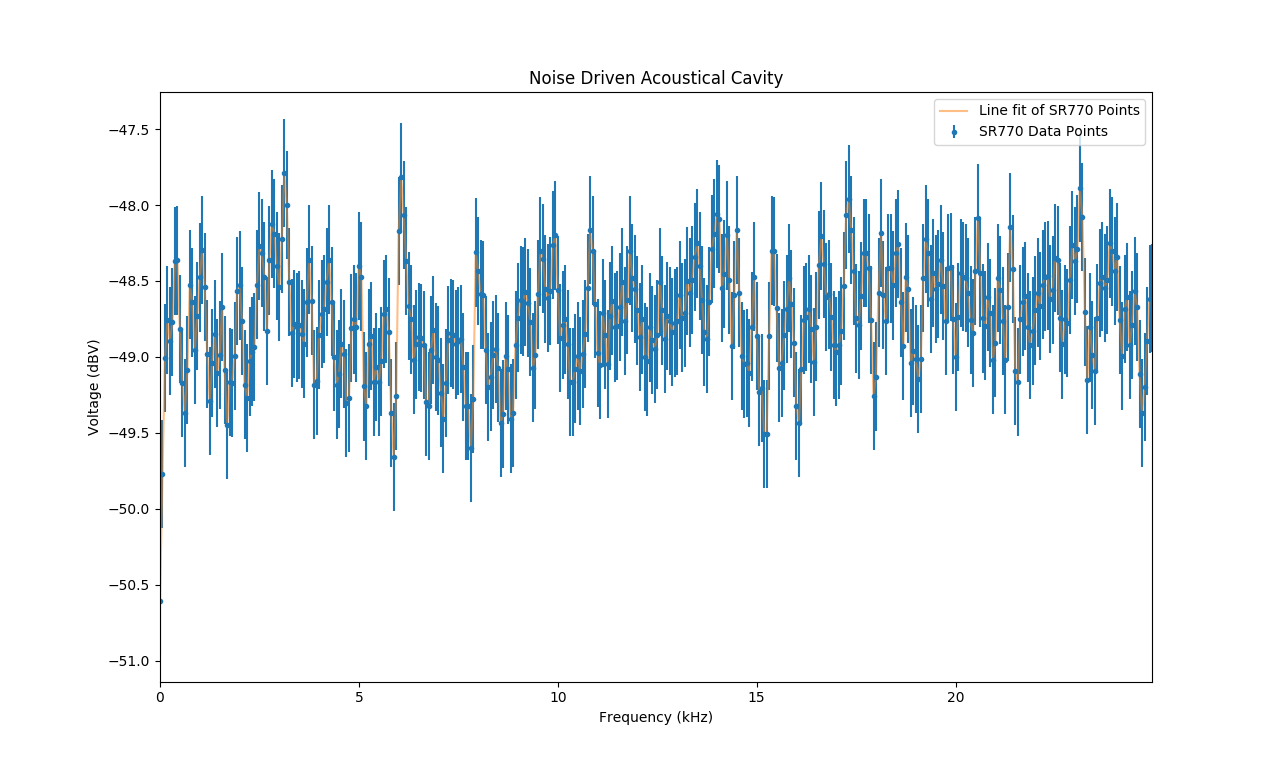
\includegraphics[width=10cm, height=6cm]{figures/figure31.png}
        \caption{Acoustical cavity driven by noise (should not look like noise)}
        \label{fig:fig31}
\end{tcolorbox}
\end{minipage}
\end{figure}

This is where the lab started to feel a bit rushed. Prior to the acoustical
cavity, we had time to read the data in and do enough processing on it to
ensure that everything looked correct before proceeding to the next section. We
also took the lecture time required to investigate the theory of the previous
sections. 

\subsubsection{Chirp Drive}%
\label{ssub:chirp_drive}

The chirp data that we collected is slightly better -- although, we were still
unable to save the phase data correctly. The magnitude spikes through the chirp
seem slightly more reasonable.

\begin{figure}[H]
    \centering
\begin{minipage}{11cm}
\begin{tcolorbox}
    \centering
        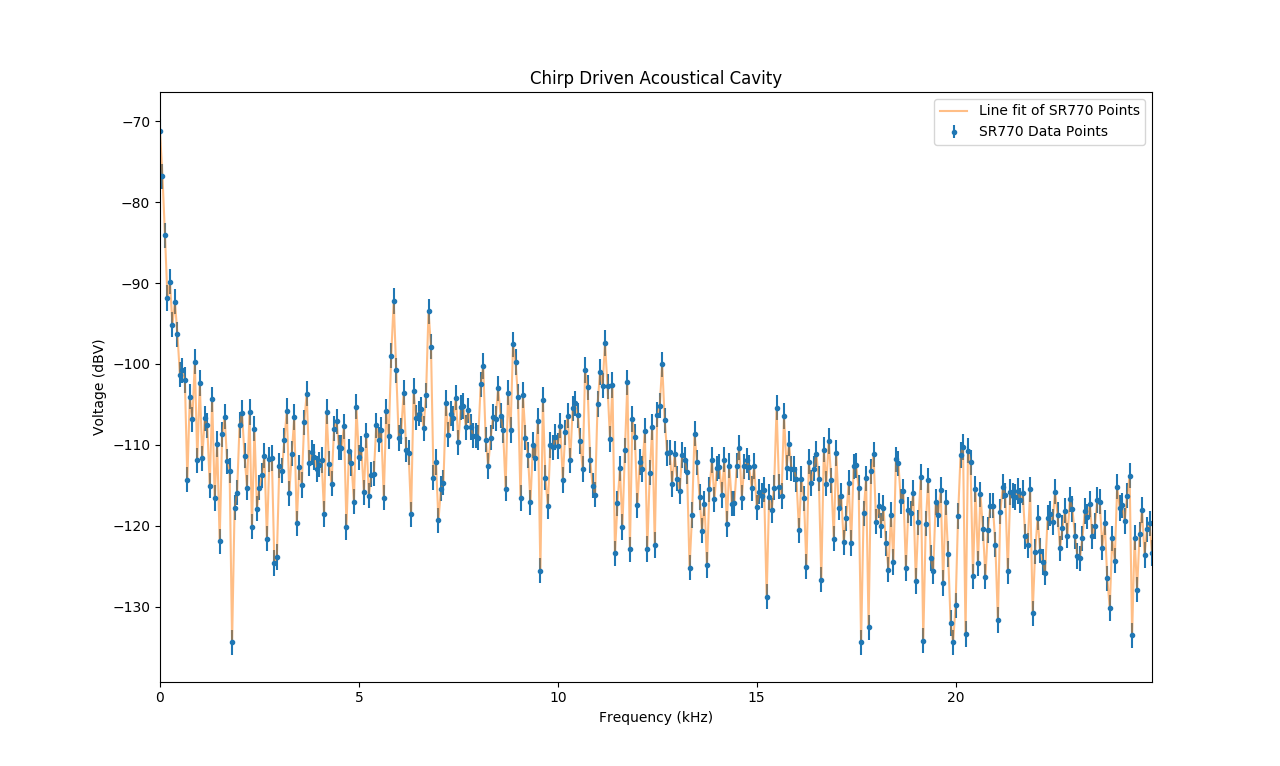
\includegraphics[width=10cm, height=6cm]{figures/figure32.png}
        \caption{Acoustical cavity chirp drive magnitude data}
        \label{fig:fig32}
\end{tcolorbox}
\end{minipage}
\end{figure}

\subsubsection{Transient Response}%
\label{ssub:transient_response}

The most interesting plot from passing a square wave through the acoustical
cavity is actually from the scope. The time domain data for a transient
response through the cavity is very characteristic of filter behavior:

\begin{figure}[H]
    \centering
\begin{minipage}{11cm}
\begin{tcolorbox}
    \centering
        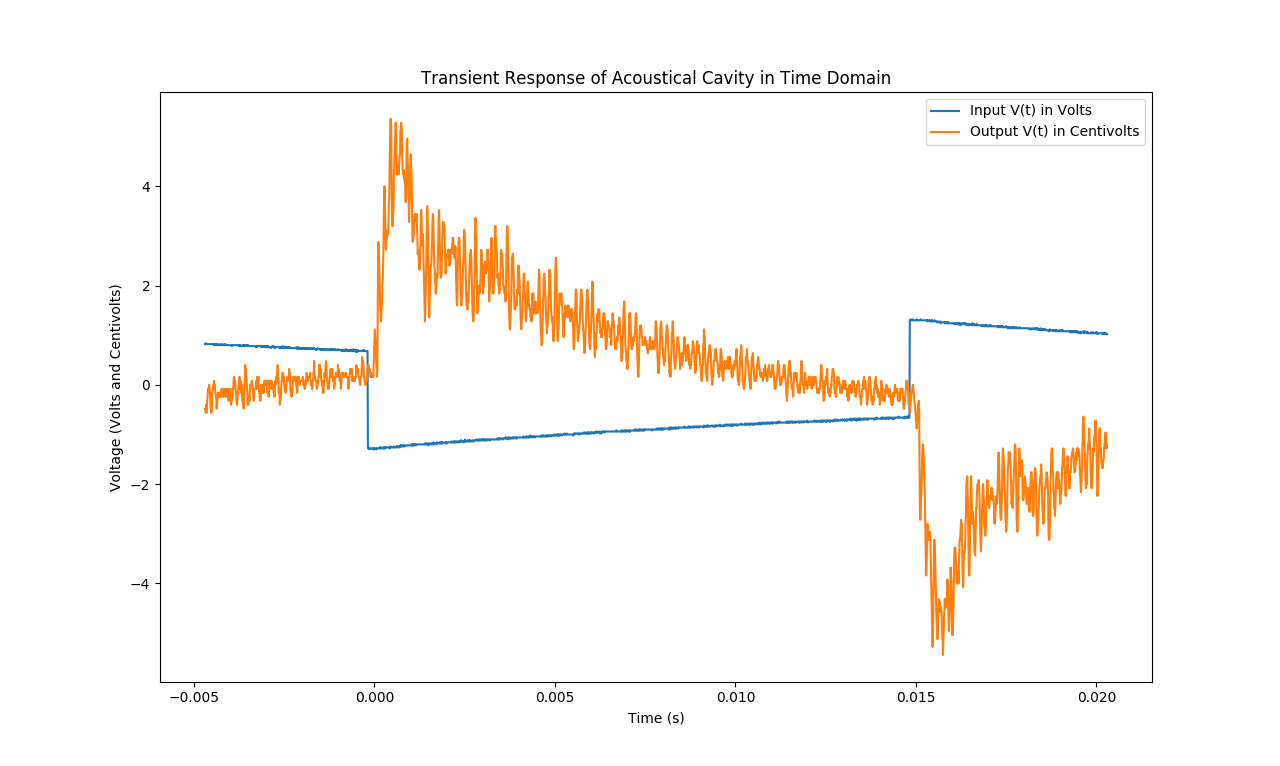
\includegraphics[width=10cm, height=6cm]{figures/figure33.png}
        \caption{Acoustical cavity transient response oscilloscope data in the
        time domain}
        \label{fig:fig33}
\end{tcolorbox}
\end{minipage}
\end{figure}

If we instead collect the frequency dependent data from the analyzer, we can
see several different peaks:

\begin{figure}[H]
    \centering
\begin{minipage}{11cm}
\begin{tcolorbox}
    \centering
        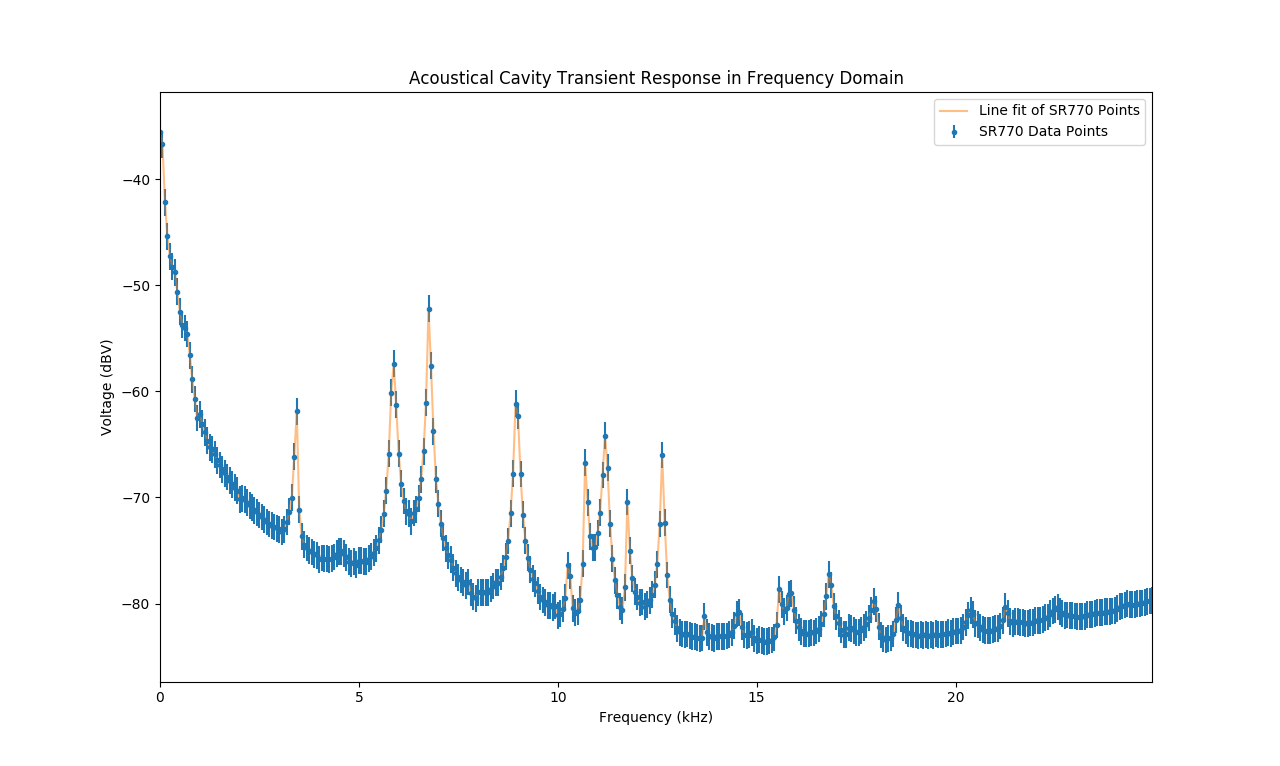
\includegraphics[width=10cm, height=6cm]{figures/figure34.png}
        \caption{Acoustical cavity transient response to 33.33 Hz square wave
        in the frequency domain}
        \label{fig:fig34}
\end{tcolorbox}
\end{minipage}
\end{figure}

\subsection{Coupled Torsional Reed Oscillators}%
\label{sub:coupled_torsional_reed_oscillators}

We ran out of time before collecting any data for this section -- however, we
did have time to play around with the system and discuss the theory with Ryan.
I have included a brief theoretical description of this in my lab notebook. As
there is no data to present, and this report is already prohibitively lengthy,
I will not reproduce the notes here. 

\section{Questions}%
\label{sec:questions}

\subsection{SR770 Normalization}%
\label{sub:sr770_normalization}

There are several different ways that the SRS is capable of normalizing the
data that it displays. For the most part, we were collecting data in the
Spectrum and PSD modes. So, hopping over to the user manual we see that the PSD
by default is 

\begin{quote}
The magnitude of the spectrum (the square root of [the FFT times its
complex conjugate]) normalized to a bandwidth of 1 Hz. This measurement
approximates the amplitude within a 1 Hz bandwidth located at each
frequency bin. The actual line width and window function are compensated for
in this calculation. This allows measurements taken with different spans or
windows to be compared.
\end{quote}

I would interpret this to mean that they normalize in the standard way to 1 Hz.
For a more detailed explanation about how frequencies are normalized during a
Fourier Transform, check out any of these sites:

\href{dsp.stackexchange.com/questions/41518/what-is-normalized-frequency}{Stack Exchange Article}

\href{matteolandi.blogspot.com/2010/08/notes-about-fft-normalization.html}{Blog Post about Normalization} 

\href{www.mathworks.com/matlabcentral/answers/15770-scaling-the-fft-and-the-ifft}{Mathworks Article} 

Alternatively, take a look at how I normalize the data from the oscilloscope.
Since my data matches the analyzer data, it is reasonable to assume that the
analyzer will normalize in a very similar method. When normalizing the voltage
(y-axis) it is important to divide by the number of points:

\begin{figure}[H]
\centering
\begin{minipage}{1\textwidth}
\begin{tcolorbox}
\begin{minted}{python}
def transformY(self):

    """Fourier Transfrom the voltage of a function
    :self.N: the number of points
    :returns: an array with the FT of the voltage of a sine
    """

    return 20 * np.log10(
            2.0/self.N *
            np.abs(fft(self.voltageFunction)[0:self.N//2]))
\end{minted}
\end{tcolorbox}
\end{minipage}
\end{figure}

Then, we can use this algorithm in order to ensure that we situate the
frequency (x-axis) bins correctly: 

\begin{figure}[H]
\centering
\begin{minipage}{1\textwidth}
\begin{tcolorbox}
\begin{minted}{python}
def transformX(self):
    """Produce the frequency bins for a single frequency wave

    :self.T: the spacing between points
    :self.N: the number of points

    :returns: An array with the frequency bins (IE the x axis)
    """

    return np.linspace(0.0, 1.0 / (2.0 * self.T), self.N//2)
\end{minted}
\end{tcolorbox}
\end{minipage}
\end{figure}


\subsection{Time Domain Usefulness}%
\label{sub:time_domain_usefulness}

Based on this lab, operating in the time domain seems to be most useful when
there are multiple frequencies present. For example, when we examined the
buried treasure module, it was possible to resolve a signal in the frequency
domain that we could not see at all in the time domain.

Additionally, it was super useful during the investigation of the transient
response (square) and sawtooth (triangle) waves because it lets you start to
pick apart the details about what is happening under the surface

\section{Code Appendix}%
\label{sec:code_appendix}

The coding aspect of this lab was extensive enough that it seemed
to warrant utilizing classes. So, I defined a class for measurements, and one
for models. Within the model class, there are numerous sub classes. I took time
to fully document the code, so it should be fairly straightforward. The goal of
this section is to provide a 30,000 foot overview and point out a couple sneaky
things. It does not aim to provide a full walk through of the code.


\subsection{Measurement Class}%
\label{sub:measurement_class}

The measurement class has several important attributes. I carry uncertainty
through all the analyzer data. Propagating error through a Fourier Transform is
outside the scope of this lab, so I do not carry it through the oscilloscope
data. After reviewing the data sheet, the analyzer is able to resolve data to
$\pm($0.3 dB + 0.02\% of full scale) where the full scale excludes window
effects and only takes into consideration the actual data points. In python,
this looks like

\begin{figure}[H]
\centering
\begin{minipage}{1\textwidth}
\begin{tcolorbox}
\begin{minted}{python}
# define the full scale of points
an_scale = \
    abs(max(self.an['voltage']) - min(self.an['voltage']))

# apply the uncertainty as an array
self.voltage = \
    pd.Series(uarray(self.an['voltage'], .3 + .02 * an_scale))
\end{minted}
\end{tcolorbox}
\end{minipage}
\end{figure}

An instance of the measurement class has access to a method for taking the
Fourier Transform. I'm not especially proud of the method, but it does get the
job done. There are a couple sneaky things. NumPy's fft method does not
automatically shift and normalize the data, so we have to do it explicitly
Additionally, using the `np.log()' method will default to the natural log. We
should use `np.log10()' instead. Lastly, we can use the `np.fftfreq()' method
to recover the frequency bins:

\begin{figure}[H]
\centering
\begin{minipage}{1\textwidth}
\begin{tcolorbox}
\begin{minted}{python}
# perform the transformation on voltage
fftvolt = np.fft.fft(self.voltage)

# clean up and normalize
fftvolt = np.fft.fftshift(fftvolt)
fftvolt = 2*fftvolt/float(len(self.voltage))

# convert voltage to dB
self.fftdbv = 20.*np.log10(np.abs(fftvolt))

# determine the time step and window length
self.time_step = self.time[2]- self.time[1]
self.win_length = len(self.time)

# recover frequency bins and shift them
self.fftfreq = np.fft.fftfreq(
    self.win_length, self.time_step)

self.fftfreq = np.fft.fftshift(self.fftfreq)
\end{minted}
\end{tcolorbox}
\end{minipage}
\end{figure}

Implementing and plotting the measurement class is very simple. For example,
let's say you want to examine the 5th measurement we made. You could create a
new .py file and fill it with:
\begin{figure}[H]
\centering
\begin{minipage}{1\textwidth}
\begin{tcolorbox}
\begin{minted}{python}
from measurement import *
data = measurement(5)
\end{minted}
\end{tcolorbox}
\end{minipage}
\end{figure}

Upon running this script, you will be greeted with a readout that provides all
the metadata regarding the 5th measurement
\begin{figure}[H]
\centering
\begin{minipage}{1\textwidth}
\begin{tcolorbox}
\begin{minted}{bash}
id    filepath form_name  channel_num  frequency  amplitude
 5   511121518      sine            1    11097.0        5.0
 ...
 5  scope-511121518 sine            2    11597.0        1.0
\end{minted}
\end{tcolorbox}
\end{minipage}
\end{figure}

From here, you should have enough information to plot the data and give it
an accurate title, label, etc. In this case the full script would be:

\begin{figure}[H]
\centering
\begin{minipage}{1\textwidth}
\begin{tcolorbox}
\begin{minted}{python}
from measurement import *
data = measurement(5)

data.model(
    title='Summing Two Sine Waves', 
    ylabel='Voltage (dB)', 
    xlabel='Frequency (kHz)', 
    plotSc=False)

plt.legend()
plt.show()
\end{minted}
\end{tcolorbox}
\end{minipage}
\end{figure}

I have caught all the errors and handled them in a way that prevent's the
module from crashing. But, let's say you can't remember the ID of the
measurement that you want to examine. You can use the `measurement.query()'
method to perform any SQL query on the database. For example, let's say you
know that the wave in which you are interested is driven by a triangle. You
could do something like

\begin{figure}[H]
\centering
\begin{minipage}{1\textwidth}
\begin{tcolorbox}
\begin{minted}{python}
from measurement import query
query('SELECT * FROM info WHERE form_name = "triangle"')
\end{minted}
\end{tcolorbox}
\end{minipage}
\end{figure}

This would print a list of all the meta data for measurements with a triangle
wave input function. From there, you could pick out the ID for which you are
looking and model the data.


\subsection{Model Class}%
\label{sub:model_class}

The model class has quite a few sub classes. All of it's sub classes have a
model method which overrides the model method. The structure is fairly
complicated, so here is a tree illustrating the relationships between sub
classes:

\begin{figure}[H]
\centering
\begin{minipage}{1\textwidth}
\begin{tcolorbox}
\begin{minted}{bash}
model
    |-----fourierModel
                |-----sine
                |-----triangle
                |-----square
                |-----sineSum
                |-----sineMult
                |-----lrc
                        |-----lrcSine
                        |-----lrcSquare
                        |-----lrcMultFreq
                                    |-----lrcMultFreqGain
                                    |-----lrcMultFreqPhase
\end{minted}
\end{tcolorbox}
\end{minipage}
\end{figure}

Implementing the model class is also very simple. Let's return to the previous
example we had. We were investigating the 5th measurement. By comparing the
file-path to my lab notebook, we can deduce that measurement 5 corresponds to
the addition module with one wave at 11.097 kHz and the other at 11.597 kHz.
Once we know that, we can examine the model classes and deduce that sineSum is
probably the correct one to use. Implementation is exactly what you would
expect:

\begin{figure}[H]
\centering
\begin{minipage}{1\textwidth}
\begin{tcolorbox}
\begin{minted}{python}
import model

mymodel = model.sineSum(
    freqA=11.097, 
    freqB=11.597, 

    # using RMS amplitudes
    ampA=(5 / (2 * np.sqrt(2)), 
    ampB=(1 / (2 * np.sqrt(2))))
)

mymodel.model()
plt.legend()
plt.show()
\end{minted}
\end{tcolorbox}
\end{minipage}
\end{figure}

The form of implementation will be identical for any of the measurements.
Auto completion suggestions are very helpful in knowing the order of the
required parameters.


\end{document}
